% =====================================================================
%  ENGR 5315 -- M.Eng. Capstone Final Report
%  Author : Tirth Shah
%  Title  : Motivational Interviewing Chatbot for Alcohol-Related Dialogues
%  Build  : pdflatex main && bibtex main && pdflatex main && pdflatex main
% =====================================================================
\documentclass[11pt,letterpaper]{article}

% ----- Page geometry -----
\usepackage[margin=1in]{geometry}
\usepackage{setspace}
\onehalfspacing

% ----- Encoding & fonts -----
\usepackage[T1]{fontenc}
\usepackage[utf8]{inputenc}
\usepackage{lmodern}
\usepackage{microtype}

% ----- Math, symbols, units -----
\usepackage{amsmath,amssymb,amsthm}
\usepackage{siunitx}

% ----- Graphics, tables -----
\usepackage{graphicx}
\graphicspath{{figures/}}
\usepackage{booktabs}
\usepackage{multirow}
\usepackage{array}
\usepackage{tabularx}
\usepackage{caption}
\captionsetup{font=small,labelfont=bf}

% ----- Diagrams (used for the runtime pipeline in methodology) -----
\usepackage{tikz}
\usetikzlibrary{positioning,arrows.meta,shapes.geometric}

% ----- Code listings -----
\usepackage{listings}
\usepackage{xcolor}
\definecolor{lstbg}{RGB}{248,248,248}
\definecolor{lstkw}{RGB}{0,0,180}
\definecolor{lststr}{RGB}{163,21,21}
\definecolor{lstcmt}{RGB}{0,128,0}
\lstset{
    basicstyle=\ttfamily\footnotesize,
    backgroundcolor=\color{lstbg},
    keywordstyle=\color{lstkw}\bfseries,
    stringstyle=\color{lststr},
    commentstyle=\color{lstcmt}\itshape,
    frame=single,
    rulecolor=\color{black!20},
    breaklines=true,
    breakatwhitespace=true,
    showstringspaces=false,
    columns=flexible,
    tabsize=2,
    captionpos=b,
}
\lstdefinelanguage{json}{
    morestring=[b]",
    morestring=[d]',
    stringstyle=\color{lststr},
    keywords={true,false,null},
    keywordstyle=\color{lstkw}\bfseries,
}

% ----- Refs & links -----
\usepackage[hidelinks,colorlinks=true,linkcolor=black,citecolor=blue!60!black,urlcolor=blue!60!black]{hyperref}
\usepackage{cleveref}

% ----- Bibliography -----
\usepackage[numbers,sort&compress]{natbib}

% ----- Header / footer -----
\usepackage{fancyhdr}
\pagestyle{fancy}
\fancyhf{}
\renewcommand{\headrulewidth}{0.4pt}
\fancyhead[L]{\small Motivational Interviewing Chatbot}
\fancyhead[R]{\small Tirth Shah \textbar{} M.Eng. Capstone}
\fancyfoot[C]{\thepage}

\title{\textbf{Motivational Interviewing Chatbot for Alcohol-Related Dialogues:\\
A Fine-Tuned, Retrieval-Augmented, Safety-Layered LLM Pipeline}}
\author{Tirth Shah\\
        \small M.Eng. in Computer Science\\
        \small University of Connecticut\\
        \small \texttt{tirthshah2812@gmail.com}}
\date{May 2026}

\begin{document}

% =====================================================================
%  TITLE PAGE
% =====================================================================
\begin{titlepage}
    \centering
    \vspace*{1cm}

    {\large UNIVERSITY OF CONNECTICUT \\[0.2em]
            College of Engineering \\
            Master of Engineering Program \\
            ENGR 5315 -- M.Eng. Capstone Project \par}

    \vspace{3cm}

    {\Huge \bfseries Motivational Interviewing Chatbot for Alcohol-Related Dialogues \par}
    \vspace{0.6cm}
    {\Large A Fine-Tuned, Retrieval-Augmented, Safety-Layered LLM Pipeline\par}

    \vspace{2.5cm}

    {\large \textbf{Tirth Shah} \par}
    \vspace{0.2cm}
    {\large \texttt{tirthshah2812@gmail.com} \par}

    \vspace{1.5cm}

    {\large \textit{Capstone Instructor} \par}
    {\large \textbf{Prof.\ Tingting Yu} \par}

    \vspace{1.5cm}

    {\large \textit{Submitted in partial fulfillment of the requirements\\
                    for the degree of Master of Engineering in Computer Science}\par}

    \vfill

    {\large May 2026 \par}
\end{titlepage}

% =====================================================================
%  FRONT MATTER
% =====================================================================
\pagenumbering{roman}

\section*{Abstract}
\addcontentsline{toc}{section}{Abstract}

High-risk alcohol use is among the most preventable health burdens worldwide, yet
the evidence-based behavioral approach to addressing it -- Motivational Interviewing
(MI) -- requires a trained counselor and does not scale. General-purpose large
language models (LLMs) appear at first to be a natural fit, but they default to
advice-giving and gentle confrontation, which is precisely what drives ambivalent
or defensive users away.

This capstone project designs, implements, and evaluates an end-to-end MI
chatbot system that addresses this gap. The contribution is not a single model
but a six-stage pipeline:
(1) input safety screening for crisis ideation and restricted topics,
(2) silent state inference scoring the user across seven emotion classes and
four defensiveness levels,
(3) retrieval-augmented generation over a curated MI knowledge base using FAISS
and \texttt{all-MiniLM-L6-v2} embeddings,
(4) response generation by a LoRA-fine-tuned \texttt{gemma-2-2b-it} served
locally through Ollama,
(5) output safety screening for medical-advice patterns, and
(6) per-turn JSONL audit logging.

The fine-tuning corpus combines the alcohol-only subset of AnnoMI~\cite{wu2022annomi}
with approximately one thousand synthetic MI conversations generated by Claude
under explicit MI guardrails. The system is evaluated using an LLM-as-judge
framework~\cite{zheng2023judging} in which Claude Sonnet scores responses on a
1--5 scale across five MI dimensions: empathy, MI technique, resistance handling,
autonomy support, and appropriateness. Across 181 evaluation items spanning real
AnnoMI turns, synthetic scenarios, and edge cases, the fine-tuned model with
RAG (\textit{v2 + RAG}) reaches an overall score of 3.81/5.0, a relative
improvement of $+17.2\%$ over the base \texttt{gemma-2-2b-it} (3.25/5.0) and
closing roughly $40\%$ of the gap to a much larger Claude Haiku reference
(4.61/5.0). The system is deployed via two interfaces -- a Streamlit
developer/evaluation app and a React + FastAPI end-user web app -- both sharing
a single Python pipeline. All conversations are auditable through structured
per-turn JSONL logs.

\noindent\textbf{Keywords:} Motivational Interviewing, large language models,
parameter-efficient fine-tuning, LoRA, retrieval-augmented generation,
LLM-as-judge evaluation, conversational safety, behavioral health.

\newpage

\tableofcontents
\newpage

\listoffigures
\listoftables
\newpage

% =====================================================================
%  BODY
% =====================================================================
\pagenumbering{arabic}
\setcounter{page}{1}

\section{Introduction and Background}
\label{sec:introduction}

\subsection{Problem Statement}

Roughly one in seven adults in the United States meets criteria for an
alcohol-use disorder in any given year, yet only a small minority ever speak to
a counselor about it~\cite{niaaa2023}. The evidence-based clinical approach to
ambivalence about substance use is \textit{Motivational Interviewing} (MI),
developed by Miller and Rollnick~\cite{miller2013mi}. MI is collaborative and
goal-oriented but explicitly non-confrontational: rather than tell the patient
what to do, the clinician helps the patient articulate their own reasons for
change.

Two facts motivate this project. First, qualified MI clinicians do not scale --
training, supervision, and licensure are slow and expensive, and access is
geographically uneven. Second, off-the-shelf LLMs do not, by default, behave
like MI counselors. They are trained on instruction-following corpora that
reward direct answers and informative explanations, so when faced with a user
who says \textit{``I don't think I drink that much''}, the modal response from
a generic assistant is to either reassure the user (a missed opportunity to
develop discrepancy) or to enumerate health risks (a frontal assault that
provokes resistance). Neither is MI.

The question this capstone addresses is therefore practical:
\begin{quote}
\textit{Can a small, locally-deployable language model be turned into a
credible Motivational Interviewing assistant for alcohol-related conversations,
with explicit safety boundaries and full conversation auditability?}
\end{quote}

\subsection{Project Goals and Objectives}

The objectives of this project, in priority order, are:
\begin{enumerate}
    \item \textbf{Behavioral fidelity.} Produce responses that visibly follow
    MI principles (express empathy, roll with resistance, support autonomy,
    develop discrepancy) rather than defaulting to advice-giving or
    information-dumping.
    \item \textbf{State awareness.} Detect when a user shifts from openness
    to defensiveness mid-conversation and adapt the response style accordingly,
    silently -- without exposing the inferred state to the user.
    \item \textbf{Safety.} Detect crisis ideation (suicidal language,
    self-harm, overdose) and restricted-topic content (medication dosing,
    prescriptions) both before \emph{and} after model inference, and
    short-circuit to evidence-based crisis resources when warranted.
    \item \textbf{Auditability.} Produce a structured, per-turn record of every
    conversation containing the inferred state, retrieved knowledge, safety
    flags, and full text -- so that the pipeline is inspectable rather than a
    black-box LLM call.
    \item \textbf{Local deployability.} Run the production model on a CPU-only
    workstation through Ollama, with a transparent fallback to a hosted API
    when local inference is unavailable.
\end{enumerate}

\subsection{Scope and Limits}

The system is a research artifact, not a clinical product. It is not validated
under an institutional review board, has not been reviewed at scale by licensed
clinicians, and is not appropriate for unsupervised deployment to people in
acute distress. Its purpose is to demonstrate the engineering of an
MI-aligned conversational pipeline and to characterize, quantitatively, what a
small fine-tuned model can reach versus a large reference model on the same
task. The honest limits of the system are stated explicitly in
\Cref{sec:future_work}.

\subsection{Report Outline}

The remainder of this report is organized as follows.
\Cref{sec:literature} surveys related work in MI, parameter-efficient
fine-tuning, retrieval-augmented generation, and LLM-as-judge evaluation.
\Cref{sec:methodology} describes the six-stage pipeline architecture and the
fine-tuning, retrieval, and safety designs.
\Cref{sec:analysis} discusses the key engineering analyses and trade-offs --
data scarcity, model size selection, evaluation design.
\Cref{sec:experiments} specifies the evaluation set, the LLM-as-judge protocol,
and the configurations compared.
\Cref{sec:results} presents quantitative and qualitative results.
\Cref{sec:conclusions} summarizes findings, and \Cref{sec:future_work} lays out
recommended future work.

\section{Survey of Related Literature}
\label{sec:literature}

This project sits at the intersection of four bodies of work: Motivational
Interviewing as a behavioral-health methodology, parameter-efficient fine-tuning
of language models, retrieval-augmented generation, and automated evaluation
of dialogue systems. The relevant prior art in each is summarized here.

\subsection{Motivational Interviewing}

Motivational Interviewing was introduced by Miller and Rollnick~\cite{miller2013mi}
as a counseling style for resolving ambivalence about behavior change. Its
operational core is the OARS skill set --
\textit{Open questions}, \textit{Affirmations}, \textit{Reflections},
\textit{Summaries} -- combined with four guiding principles:
\textit{express empathy}, \textit{develop discrepancy}, \textit{roll with
resistance}, and \textit{support self-efficacy}. Meta-analytic evidence supports
MI as an effective intervention for alcohol-use disorders compared to no-treatment
controls, with effect sizes that, while modest, are robust across populations
and settings~\cite{lundahl2010metaanalysis}.

The empirical literature on \emph{automating} MI-aligned dialogue is much
younger. Wu et al.~\cite{wu2022annomi} introduced the AnnoMI corpus -- the only
publicly available dataset of expert-annotated MI transcripts -- and a baseline
classifier for MI-consistent versus MI-inconsistent turns. AnnoMI is the
real-data backbone of this project.

\subsection{Parameter-Efficient Fine-Tuning}

Full fine-tuning of multi-billion-parameter language models is prohibitive on
single-GPU consumer hardware. Hu et al.~\cite{hu2022lora} introduced
\textbf{Low-Rank Adaptation (LoRA)}, which freezes the pretrained weight matrix
$W \in \mathbb{R}^{d \times k}$ and learns a low-rank update
$\Delta W = BA$ where $B \in \mathbb{R}^{d \times r}$ and
$A \in \mathbb{R}^{r \times k}$, with $r \ll \min(d,k)$. LoRA reduces trainable
parameters by orders of magnitude while matching full-fine-tuning quality on
GLUE-scale benchmarks. Dettmers et al.~\cite{dettmers2023qlora} extended this
to QLoRA, in which the frozen base model is quantized to 4-bit precision so that
even very large models fit on a single consumer GPU.

This project uses LoRA via the Hugging Face PEFT library~\cite{peft2023}, applied
to all attention and MLP projection matrices of \texttt{gemma-2-2b-it}, with the
base weights kept in 4-bit NF4 precision during training. The Gemma model
family itself was released by Google~\cite{gemma2024}, with the 2B-instruct
checkpoint chosen here for local deployability.

\subsection{Retrieval-Augmented Generation}

Lewis et al.~\cite{lewis2020rag} introduced \textbf{Retrieval-Augmented Generation
(RAG)} as a method for grounding language model outputs in non-parametric
knowledge: at inference time, an embedding-based retriever fetches the
$k$ most relevant passages from a document store and concatenates them to the
prompt. RAG mitigates hallucination and lets the system update its knowledge
without retraining the model.

The retrieval component of this project uses FAISS~\cite{johnson2019faiss} as
the approximate-nearest-neighbor index and \texttt{all-MiniLM-L6-v2}~\cite{reimers2019sentencebert}
as the encoder. \texttt{all-MiniLM-L6-v2} was selected over larger encoders for
its $\approx 30 \times$ speed advantage on CPU and its strong retrieval quality
on the MTEB benchmark~\cite{muennighoff2022mteb} relative to its size.

\subsection{LLM-as-Judge Evaluation}

Evaluating open-ended dialogue is a long-standing problem. Reference-based
metrics such as BLEU and ROUGE correlate poorly with human judgement on tasks
where many distinct responses are valid~\cite{liu2016how}. Human evaluation is
the gold standard but is too slow to drive an iteration loop on a one-person
project.

Zheng et al.~\cite{zheng2023judging} demonstrated that strong LLMs (GPT-4,
Claude) used as judges achieve $80\%+$ agreement with human raters on
chatbot-arena-style pairwise judgements, comparable to inter-human agreement.
Subsequent work~\cite{chiang2023closer} showed that the LLM-as-judge protocol
is sensitive to position bias, verbosity bias, and self-preference bias, and
recommends mitigations including symmetric pairwise prompting and explicit
rubrics. This project applies the rubric variant -- the judge sees a fixed
five-dimension MI rubric and produces calibrated 1--5 scores -- and treats the
results as a coarse iteration signal rather than ground truth, in line with
the recommendations of \cite{chiang2023closer}.

\subsection{Conversational Safety}

Safety in deployed conversational AI is typically implemented as a
defense-in-depth stack: input filtering, in-context guardrails inside the
prompt, post-generation classifiers, and audit logging~\cite{markov2023moderation,inan2023llamaguard}.
This project adopts a stripped-down version of that pattern -- a regex-based
input and output screen for crisis and medical-boundary content, plus per-turn
JSONL audit logging -- chosen explicitly because it is auditable line-by-line,
which an embedding-based classifier is not.

\section{Methodology}
\label{sec:methodology}

\subsection{System Overview}

The system is a six-stage Python pipeline shared by two front ends. Every user
message is run through the same pipeline; only the presentation layer differs
between the developer/evaluation interface and the end-user web interface.
\Cref{fig:pipeline} shows the runtime path of a single turn.

\begin{figure}[t]
\centering
\begin{minipage}{0.95\linewidth}
\centering
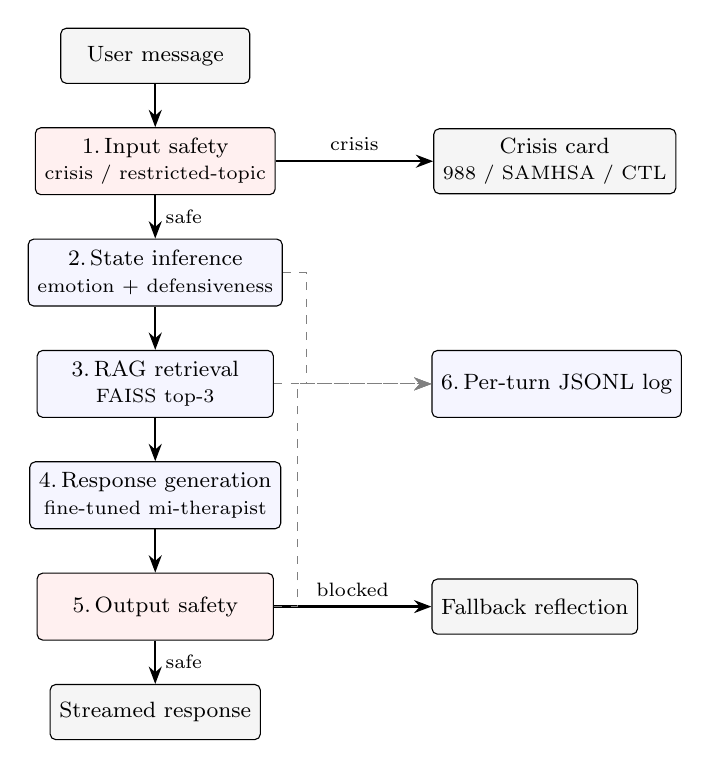
\begin{tikzpicture}[
    node distance=0.55cm and 0.65cm,
    every node/.style={font=\footnotesize},
    box/.style={draw, rounded corners=2pt, align=center, minimum width=3.0cm,
                minimum height=0.85cm, fill=blue!4},
    safe/.style={draw, rounded corners=2pt, align=center, minimum width=3.0cm,
                 minimum height=0.85cm, fill=red!6},
    io/.style={draw, rounded corners=2pt, align=center, minimum width=2.4cm,
               minimum height=0.7cm, fill=gray!8},
    arr/.style={-{Stealth[length=2.2mm]}, thick},
    side/.style={-{Stealth[length=2.2mm]}, dashed, gray}
]
\node[io] (u) {User message};
\node[safe, below=of u] (s1) {1.\,Input safety \\ \scriptsize crisis / restricted-topic};
\node[box, below=of s1] (st) {2.\,State inference \\ \scriptsize emotion + defensiveness};
\node[box, below=of st] (rag) {3.\,RAG retrieval \\ \scriptsize FAISS top-3};
\node[box, below=of rag] (rg) {4.\,Response generation \\ \scriptsize fine-tuned mi-therapist};
\node[safe, below=of rg] (s2) {5.\,Output safety};
\node[io, below=of s2] (out) {Streamed response};

\node[io, right=2.0cm of s1] (cr) {Crisis card \\ \scriptsize 988 / SAMHSA / CTL};
\node[io, right=2.0cm of s2] (fb) {Fallback reflection};
\node[box, right=2.0cm of rag] (log) {6.\,Per-turn JSONL log};

\draw[arr] (u) -- (s1);
\draw[arr] (s1) -- node[right,font=\scriptsize]{safe} (st);
\draw[arr] (s1) -- node[above,font=\scriptsize]{crisis} (cr);
\draw[arr] (st) -- (rag);
\draw[arr] (rag) -- (rg);
\draw[arr] (rg) -- (s2);
\draw[arr] (s2) -- node[right,font=\scriptsize]{safe} (out);
\draw[arr] (s2) -- node[above,font=\scriptsize]{blocked} (fb);

\draw[side] (st.east) -- ++(0.3,0) |- (log.west);
\draw[side] (rag.east) -- (log.west);
\draw[side] (s2.east) -- ++(0.3,0) |- (log.west);
\end{tikzpicture}
\end{minipage}
\caption{Six-stage runtime pipeline. Solid arrows are the request path; dashed
arrows indicate side-effect writes to the per-turn audit log. Stages 1 and 5
are red because they can short-circuit the pipeline; the remaining stages
always execute when the input passes the input safety check.}
\label{fig:pipeline}
\end{figure}

The orchestrator is \texttt{ConversationManager}, which owns a
\texttt{ConversationHistory}, a \texttt{StateInferencer}, a
\texttt{RAGPipeline}, a \texttt{ResponseGenerator}, and a
\texttt{ConversationLogger}. The same object graph is wrapped by either the
Streamlit dev/eval app (\texttt{app.py}) or the FastAPI server
(\texttt{backend\_server.py}).

\subsection{Stage 1 -- Input Safety}

The input safety layer (\texttt{src/safety\_layer.py}) screens the incoming
user message for two categories of content:

\begin{itemize}
    \item \textbf{Crisis indicators.} Suicidal ideation (active and passive),
    self-harm intent, and overdose. Patterns include direct phrases
    (``kill myself'', ``end it'') and indirect phrasings (``no reason to
    keep going'', ``don't even want to be here''). The original implementation
    used strict-adjacency regexes; these missed many natural phrasings, so the
    patterns were broadened with optional-intensifier groups during late-stage
    polish.
    \item \textbf{Restricted topics.} Medication dosing and prescription
    advice. The system is not a clinical authority; it is explicitly designed
    to refuse this category of request.
\end{itemize}

A crisis match short-circuits the entire pipeline -- no RAG retrieval, no LLM
call, just a pre-written response containing the 988 Suicide \& Crisis
Lifeline, SAMHSA helpline, and Crisis Text Line. A restricted-topic match
returns a medical-boundary response with the same short-circuit.

The choice of regex over an embedding-based classifier is deliberate: every
trigger is auditable line-by-line, and the cost of a false negative here is
much higher than the cost of a false positive.

\subsection{Stage 2 -- State Inference}

The state inferencer (\texttt{src/state\_inference.py}) scores each user
message on two axes:

\begin{itemize}
    \item \textbf{Emotion} -- one of seven classes:
    \textit{neutral}, \textit{frustrated}, \textit{anxious}, \textit{sad},
    \textit{angry}, \textit{hopeful}, \textit{contemplative}.
    \item \textbf{Defensiveness} -- one of four levels:
    \textit{none}, \textit{low}, \textit{moderate}, \textit{high}.
\end{itemize}

For local Gemma runs the inference is rule-based using weighted regular
expressions over linguistic markers (modal verbs, hedging, negations, intensity
words), which runs in $\sim$30~ms. For API runs an LLM call is used instead.
Either path produces the same JSON structure, which is consumed downstream.

The inferred state \emph{never appears in the response surface}. It is used
silently to weight retrieval and to select among prompt-template variants.
This is a deliberate UX decision -- being told ``I detect that you are
defensive'' would itself be MI-inconsistent.

\subsection{Stage 3 -- Retrieval-Augmented Generation}

The retrieval component (\texttt{src/rag\_pipeline.py}) maintains a FAISS index
over a curated MI knowledge base. The corpus consists of nine markdown
documents authored for this project plus an extracted set of high-quality MI
exchanges from AnnoMI (\Cref{tab:kb-contents}).

\begin{table}[h]
\centering
\caption{Contents of the MI knowledge base used for retrieval.}
\label{tab:kb-contents}
\begin{tabular}{ll}
\toprule
\textbf{Document} & \textbf{Purpose} \\
\midrule
\texttt{mi\_principles.md}              & Four guiding MI principles \\
\texttt{oars\_detailed\_guide.md}       & OARS skill set with examples \\
\texttt{mi\_antipatterns.md}            & What NOT to say \\
\texttt{handling\_resistance.md}        & Roll-with-resistance strategies \\
\texttt{defensiveness\_playbook.md}     & Tactics by defensiveness level \\
\texttt{stage\_of\_change\_strategies.md} & Stage-matched interventions \\
\texttt{emotional\_responses.md}        & Reflection patterns by emotion \\
\texttt{harm\_reduction.md}             & Harm-reduction framings \\
\texttt{crisis\_protocols.md}           & Escalation and resource scripts \\
\texttt{annomi\_examples/}              & Curated AnnoMI excerpts \\
\bottomrule
\end{tabular}
\end{table}

The configuration is:
\begin{itemize}
    \item \textbf{Encoder.} \texttt{sentence-transformers/all-MiniLM-L6-v2}
    (384-dim, English-only).
    \item \textbf{Chunking.} \texttt{chunk\_size = 500} characters,
    \texttt{overlap = 50}.
    \item \textbf{Index.} FAISS \texttt{IndexFlatL2} (exact, sufficient given
    the small corpus size).
    \item \textbf{Retrieval.} Top-$k$ with $k=3$, biased by inferred state --
    e.g., a turn scored as ``high'' defensiveness oversamples the
    \texttt{handling\_resistance.md} and \texttt{defensiveness\_playbook.md}
    chunks instead of empathy reflections.
\end{itemize}

The retrieved chunks are injected into the prompt as ``context-specific
guidance'' in stage 4.

\subsection{Stage 4 -- Response Generation}

The response generator (\texttt{src/response\_generator.py}) builds the final
prompt as the concatenation of:
\begin{enumerate}
    \item a system message describing MI principles and style guidelines,
    \item the top-3 retrieved knowledge chunks,
    \item a sliding context window of recent dialogue turns,
    \item the new user message.
\end{enumerate}

The prompt is sent to the fine-tuned \texttt{mi-therapist} model running on
Ollama. If Ollama is unreachable, the system falls back transparently to
Claude Haiku via the Anthropic API, with the fallback fact recorded in the
audit log.

\subsubsection*{Fine-Tuning Configuration}

\begin{table}[h]
\centering
\caption{Fine-tuning configuration. ``Effective batch size'' is
$1 \times 8 = 8$; ``trainable params'' figure depends on rank and target modules.}
\label{tab:finetune-config}
\begin{tabular}{ll}
\toprule
\textbf{Parameter} & \textbf{Value} \\
\midrule
Base model              & \texttt{google/gemma-2-2b-it} \\
Quantization (training) & 4-bit NF4 (QLoRA-style) \\
Method                  & LoRA via PEFT \\
LoRA rank $r$           & 16 \\
LoRA $\alpha$           & 32 \\
LoRA dropout            & 0.05 \\
Target modules          & \texttt{q\_proj, k\_proj, v\_proj, o\_proj}, \\
                        & \texttt{gate\_proj, up\_proj, down\_proj} \\
Optimizer               & paged\_adamw\_8bit \\
Learning rate           & $2 \times 10^{-4}$ \\
Scheduler               & cosine with $10\%$ warmup \\
Epochs                  & 3 \\
Batch size              & 1 (per device) \\
Gradient accumulation   & 8 \\
Precision               & bf16 \\
Gradient checkpointing  & enabled \\
Max sequence length     & 2048 tokens \\
Hardware                & Google Colab T4 (16 GB) \\
\bottomrule
\end{tabular}
\end{table}

The trained adapters are merged back into the base weights and exported to
4-bit GGUF (Q4\_K\_M) for inference, producing a $\approx$1.6~GB artifact that
runs on a CPU through Ollama with $\sim$2--4~s per-turn latency.

\subsection{Stage 5 -- Output Safety}

After generation, the response is screened a second time for medical-advice
patterns (``you should take'', ``I recommend stopping'', explicit dosage
references). If matched, the LLM output is replaced with a generic reflective
fallback. This stage exists because system-prompt guardrails alone are not
reliable -- a fine-tuned model can still drift, especially on adversarial
inputs.

\subsection{Stage 6 -- Audit Logging}

The \texttt{ConversationLogger} writes one JSONL record per turn under
\texttt{logs/<session\_id>.jsonl} containing: timestamp, user message,
bot response, inferred state (emotion, defensiveness, reasoning, linguistic
markers), safety level, retrieved chunks. Crisis-flagged turns are
additionally appended to \texttt{logs/flagged\_for\_review.jsonl} for manual
review. The audit log is the artifact that makes the pipeline inspectable
rather than a black box.

\subsection{Two Interfaces, One Pipeline}

The same \texttt{ConversationManager} powers both UIs. \Cref{tab:two-ui}
contrasts them.

\begin{table}[h]
\centering
\caption{The same backend pipeline is wrapped by two different front ends.}
\label{tab:two-ui}
\renewcommand{\arraystretch}{1.15}
\begin{tabularx}{\linewidth}{l X X}
\toprule
 & \textbf{End-user web app} & \textbf{Developer / eval app} \\
\midrule
Entry point          & \texttt{backend\_server.py} + React frontend & \texttt{app.py} (Streamlit) \\
Stack                & FastAPI + React 18 (UMD) + Babel Standalone & Streamlit \\
Surfaces internal state? & No -- clean conversation only & Yes -- model picker, detected emotion, retrieval count, JSON debug panel \\
Crisis handling      & Soft inline card with 988 / SAMHSA / CTL & Long-form text response \\
Audience             & Non-technical demos, prof review & Engineering iteration and evaluation \\
\bottomrule
\end{tabularx}
\end{table}

The split exists because the visibility a developer needs (raw inferred state,
retrieved chunks, fallback indicator) is the same visibility an end user should
\emph{not} see -- it would break the conversational illusion that MI requires.

\subsection{Project Layout}

\Cref{fig:layout} maps the runtime pipeline to the source tree.

\begin{figure}[h]
\centering
\begin{minipage}{0.92\linewidth}
\begin{lstlisting}[basicstyle=\ttfamily\scriptsize, frame=single, backgroundcolor=\color{lstbg}]
src/                          # Runtime pipeline (shared by both UIs)
  conversation_manager.py     # Orchestrator
  state_inference.py          # Stage 2: emotion + defensiveness
  rag_pipeline.py             # Stage 3: FAISS-based retrieval
  response_generator.py       # Stage 4: adaptive prompt construction
  safety_layer.py             # Stages 1 and 5 + Stage 6 logging
  config.py

backend_server.py             # FastAPI server (end-user web app)
app.py                        # Streamlit dev/evaluation app

capstone-chatbot-design/      # End-user web frontend (React + Babel)
scripts/                      # Offline data + eval pipelines
notebooks/                    # Fine-tuning + inference notebooks
knowledge_base/               # MI guidelines + AnnoMI excerpts
data/                         # Processed datasets, synthetic batches, eval results
models/                       # (gitignored) GGUF weights + Ollama Modelfile
logs/                         # (gitignored) per-session JSONL audit logs
\end{lstlisting}
\end{minipage}
\caption{Project layout. The \texttt{src/} package is the runtime, sharable
between front ends; \texttt{scripts/} and \texttt{notebooks/} are offline.}
\label{fig:layout}
\end{figure}

\section{Analysis}
\label{sec:analysis}

This section covers the engineering analyses that drove the major design
choices: how to handle MI-data scarcity, how to choose a base model size, how
to design an evaluation that actually informed iteration, and how to structure
safety so it stayed auditable.

\subsection{Data Scarcity and Synthetic Augmentation}

The first practical constraint was data. AnnoMI~\cite{wu2022annomi}, the only
public corpus of expert-annotated MI dialogue, contains 133 transcripts across
multiple behavioral-health domains. The alcohol-only filter reduces this to a
small slice -- after preprocessing into the project's instruction-tuning
format, only $\approx$363 training and $\approx$40 evaluation examples remain.
That is not enough material on which to train a small language model to
exhibit a consistent stylistic identity.

The choice was either to (a) train on the alcohol slice as-is and accept
overfit-style brittleness, (b) widen the source to other AnnoMI domains and
introduce off-topic drift, or (c) generate additional in-domain MI dialogue
synthetically. Option (c) was selected. The synthetic generator
(\texttt{scripts/generate\_synthetic\_data.py}) prompts Claude to simulate both
sides of a counseling session, parameterized by scenario type:

\begin{itemize}
    \item \textbf{short} -- single-turn exchange,
    \item \textbf{medium} -- 3--5 turns,
    \item \textbf{long} -- 8--12 turns,
    \item \textbf{mixed defensiveness} -- the user shifts between open and
    resistant within a single conversation.
\end{itemize}

The generator prompt embeds explicit MI guardrails: no advice-giving, no
closed questions where open ones would do, the simple-then-complex reflection
pattern, varied openers to prevent template collapse. Generation was run
in batches of $\approx$50--100 conversations and saved as JSONL under
\texttt{data/synthetic/}, then deduplicated and merged with the AnnoMI subset.

The trade-off is honest: synthetic data is generated by a model that does not
itself experience ambivalence, so the simulated client side is a stylized
imitation rather than a faithful reproduction of human ambivalence. The
evidence from evaluation (\Cref{sec:results}) is that despite this limitation,
the augmented training set substantially improves response style on real
AnnoMI test turns -- so the synthetic dialogues are at least teaching the
right output distribution.

\subsection{Model Size and Local Deployability}

A second decision was the base model. The constraint of running locally on
a CPU through Ollama eliminated 7B-and-up models for interactive latency
reasons. Among the small instruction-tuned families available at project
start, three were candidates: \texttt{Llama-3.2-1B-Instruct},
\texttt{Phi-3-mini-4k-Instruct} (3.8B), and \texttt{Gemma-2-2b-it}.
Gemma-2-2B was selected on three grounds:
\begin{enumerate}
    \item \textbf{Quantization quality.} Gemma-2 quantizes to 4-bit GGUF with
    minimal observable degradation on the project's eval set, an expected
    outcome given Gemma's training-side quantization-friendliness.
    \item \textbf{License.} Permissive enough for an academic capstone that
    redistributes a fine-tuned variant.
    \item \textbf{Tooling.} First-class support in PEFT, in TRL's SFTTrainer,
    and in Ollama as a target format.
\end{enumerate}

The 2B size yielded $\approx$1.6~GB GGUF after Q4\_K\_M quantization, with
$\sim$2--4~s per-turn latency on a CPU. Larger models would close more of the
quality gap to Claude (\Cref{sec:results}) but at a latency cost that breaks
the conversational feel.

\subsection{Evaluation Design}

The single most important methodological decision was committing to LLM-as-judge
evaluation rather than human ratings. Human MI scoring requires trained raters,
$\approx$5--10 minutes per dialogue for high-quality annotation, and inter-rater
adjudication. None of that fits the iteration loop of a one-person semester
project.

The judge is Claude Sonnet, prompted with a fixed five-dimension rubric
(empathy, MI technique, resistance handling, autonomy support, appropriateness),
each scored 1--5 with a written rationale. The rubric is reproduced in
\Cref{sec:experiments}. Three design choices follow from the recommendations
of Chiang and Lee~\cite{chiang2023closer} on LLM-judge bias:
\begin{itemize}
    \item \textbf{Rubric-based, not pairwise.} Pairwise judgements are
    susceptible to position bias and verbosity bias; absolute scoring against
    a rubric is more robust at the cost of less calibrated individual scores.
    Since the goal here is comparing configurations \emph{against the same
    rubric}, absolute scoring is sufficient.
    \item \textbf{Held-out judge.} The judge model (Claude Sonnet) is from a
    different provider than any system-under-test other than the Claude Haiku
    reference; this avoids the most pathological self-preference bias.
    \item \textbf{Coarse signal, not ground truth.} The scores are treated as
    an iteration signal. Configurations are not declared ``better'' on the
    basis of a $0.05$ difference; only effects large enough to be visible to
    a human reader are emphasized in \Cref{sec:results}.
\end{itemize}

\subsection{Safety as an Auditable Layer}

The safety design uses regex rather than an embedding classifier. The argument
for an embedding model is generalization -- it would catch crisis ideation
phrased in ways the regex misses. The argument against, in this setting, is
auditability: a regex pattern list is line-by-line inspectable, and a regression
in coverage is a one-line diff. An embedding-based classifier on the same
problem requires either a labeled crisis corpus (which the project does not
have) or an off-the-shelf classifier whose decision boundaries are not
inspectable.

The cost of the regex choice was made visible mid-project: the original
patterns required strict adjacency between intent words and self-references,
so phrasings like ``don't even want to be here'' were missed. The fix was
adding optional-intensifier groups to the patterns -- a one-commit change.
That fix would not have been a one-commit change against an opaque classifier.

The defense in depth is the audit log. Even in cases where the regex misses
a borderline phrasing, the per-turn JSONL record allows after-the-fact
discovery of the miss, which an embedding classifier would not provide.

\subsection{What This Analysis Yielded}

The analyses above produced four concrete commitments that shaped the rest of
the project:
\begin{itemize}
    \item Synthetic data is part of training, not just real AnnoMI.
    \item The base model is Gemma-2-2B, not anything larger.
    \item The eval is LLM-as-judge with a rubric, run on a mixed test set
    spanning real AnnoMI turns, synthetic scenarios, and edge cases.
    \item Safety is a two-stage regex screen with audit logging, not an
    embedding classifier.
\end{itemize}

Each of these is revisited in \Cref{sec:future_work} with the cases under
which it should be reconsidered.

\section{Experimental Setup}
\label{sec:experiments}

This section specifies the data, the evaluation protocol, and the
configurations compared. The numerical results are deferred to
\Cref{sec:results}.

\subsection{Datasets}

\subsubsection*{Training data}
Training combines two sources, merged into a single instruction-tuned JSONL:
\begin{itemize}
    \item \textbf{AnnoMI alcohol-only subset.} Filtered from the full AnnoMI
    corpus~\cite{wu2022annomi} to dialogues whose declared topic is alcohol use,
    converted into instruction/response pairs for SFT. After preprocessing,
    363 training examples and 40 held-out evaluation examples remain.
    \item \textbf{Synthetic MI conversations.} Generated by the pipeline
    described in \Cref{sec:analysis} and stored as 13 batch JSONL files under
    \texttt{data/synthetic/}, totalling approximately one thousand
    conversations across short, medium, long, and mixed-defensiveness
    scenario types.
\end{itemize}

\subsubsection*{Knowledge base for retrieval}
The retrieval corpus is described in \Cref{tab:kb-contents}. It is held strictly
separate from the training corpus, so retrieved content is not memorized text
the model has already seen during fine-tuning.

\subsubsection*{Evaluation set}
The evaluation set contains 181 user turns drawn from three sources:
\begin{itemize}
    \item $\sim$80 real AnnoMI turns (held out from training),
    \item $\sim$80 synthetic eval turns spanning emotion $\times$ defensiveness
    combinations,
    \item $\sim$20 hand-crafted edge cases (deeply ambivalent, sarcastic,
    minimizing, and crisis-adjacent phrasings).
\end{itemize}
Each item provides a user turn, a reference response (where available), and
metadata for analysis (emotion, defensiveness, talk type).

\subsection{Configurations Compared}

Five configurations are evaluated on the same set of user turns. Each
configuration produces a single response per turn, scored independently by
the judge.

\begin{table}[h]
\centering
\caption{Configurations under evaluation. RAG denotes retrieval over the MI
knowledge base described in \Cref{tab:kb-contents}.}
\label{tab:configs}
\begin{tabular}{lll}
\toprule
\textbf{Tag} & \textbf{Model} & \textbf{Augmentation} \\
\midrule
\texttt{base}    & \texttt{gemma-2-2b-it} (no fine-tune) & system prompt only \\
\texttt{v1}      & Gemma-2 LoRA, AnnoMI only             & system prompt only \\
\texttt{v2}      & Gemma-2 LoRA, AnnoMI + synthetic      & system prompt only \\
\texttt{v2\_rag} & Gemma-2 LoRA, AnnoMI + synthetic      & system prompt + RAG \\
\texttt{claude}  & Claude Haiku via Anthropic API        & system prompt only \\
\bottomrule
\end{tabular}
\end{table}

\texttt{base} is the no-fine-tune ablation; \texttt{v1} isolates the effect of
adding fine-tuning on real-only data; \texttt{v2} isolates the effect of
adding synthetic data; \texttt{v2\_rag} adds retrieval on top of \texttt{v2};
and \texttt{claude} is a much larger reference model that gives an upper-bound
sense of what is achievable on the same task without size constraints.

\subsection{Evaluation Protocol}

Each configuration's response is independently scored by Claude Sonnet
(\texttt{claude-sonnet-4-6}) acting as judge, using the rubric in
\Cref{tab:rubric}. The judge is given the user turn, the model response, and
the reference response (when available), and is instructed to produce a
1--5 integer score on each of five dimensions, plus a free-text rationale and
a tag for the detected MI technique.

\begin{table}[h]
\centering
\caption{Five-dimension MI rubric used by the judge model. Each dimension is
scored 1--5, where 1 = absent or counterproductive and 5 = expert-level.}
\label{tab:rubric}
\begin{tabularx}{\linewidth}{l X}
\toprule
\textbf{Dimension} & \textbf{What it measures} \\
\midrule
\textit{Empathy}              & Does the response acknowledge the user's emotional state without minimizing or pathologizing it? \\
\textit{MI technique}         & Does the response apply OARS (open question, affirmation, reflection, summary) appropriately for the turn? \\
\textit{Resistance handling}  & When the user is defensive, does the response roll with resistance instead of arguing? \\
\textit{Autonomy support}     & Does the response leave choices to the user rather than directing them? \\
\textit{Appropriateness}      & Is the response calibrated in length, tone, and content for the user's stated context? \\
\bottomrule
\end{tabularx}
\end{table}

\subsubsection*{Why Claude Sonnet as judge}
Sonnet is from a different provider than the systems under test except for
\texttt{claude} (Haiku); this minimizes the most pathological self-preference
bias~\cite{chiang2023closer}. The Haiku reference is therefore the
configuration most exposed to bias, which is acceptable because it is being
used as an upper-bound reference rather than a configuration competing for the
``best'' label.

\subsubsection*{What is reported}
For each configuration, mean scores per dimension and an overall mean
(unweighted average across dimensions) are reported. Sample standard
deviations across the 181 items are reported in \Cref{sec:results} where
relevant. Item-level technique distributions are also reported, since they
characterize \emph{what} the model is doing differently, not just
\emph{how well} it scored.

\section{Results and Discussion}
\label{sec:results}

This section presents the evaluation results, compares the configurations
across MI dimensions, and discusses what the numbers mean qualitatively.
All scores are produced by the LLM-as-judge protocol described in
\Cref{sec:experiments}.

\subsection{Overall Scores}

\Cref{tab:results-main} reports per-dimension means and the unweighted overall
mean across the five configurations. Standard deviations are reported alongside
the means; $n$ is the number of scored items per configuration (small
differences in $n$ reflect generation failures retried but not re-scored, and
five additional edge cases scored only on the Claude reference).

\begin{table}[h]
\centering
\caption{Mean scores ($\mu \pm \sigma$) per MI dimension, by configuration.
Each cell is over $n$ test items; the rightmost column is the unweighted mean
across the five dimensions.}
\label{tab:results-main}
\small
\setlength{\tabcolsep}{4pt}
\begin{tabular}{l c c c c c c c}
\toprule
\textbf{Config} & $n$ & \textbf{Empathy} & \textbf{MI tech.} & \textbf{Resist.} & \textbf{Auton.} & \textbf{Approp.} & \textbf{Overall} \\
\midrule
\texttt{base}    & 181 & $3.11 \pm 0.80$ & $2.96 \pm 0.80$ & $3.65 \pm 0.80$ & $3.73 \pm 0.60$ & $2.78 \pm 0.83$ & $3.25$ \\
\texttt{v1}      & 181 & $3.22 \pm 0.87$ & $2.96 \pm 0.90$ & $3.52 \pm 1.01$ & $3.66 \pm 0.81$ & $2.74 \pm 0.95$ & $3.22$ \\
\texttt{v2}      & 181 & $3.44 \pm 0.97$ & $3.27 \pm 0.92$ & $3.87 \pm 1.06$ & $3.89 \pm 0.90$ & $2.92 \pm 1.09$ & $3.48$ \\
\texttt{v2\_rag} & 180 & $3.49 \pm 1.10$ & $3.85 \pm 1.08$ & $4.03 \pm 1.15$ & $4.05 \pm 0.99$ & $3.61 \pm 1.30$ & $\mathbf{3.81}$ \\
\texttt{claude}  & 186 & $4.73 \pm 0.46$ & $4.56 \pm 0.53$ & $4.82 \pm 0.46$ & $4.57 \pm 0.56$ & $4.36 \pm 0.72$ & $\mathbf{4.61}$ \\
\bottomrule
\end{tabular}
\end{table}

\Cref{fig:overall} visualizes the overall column. The fine-tuned model with
RAG closes $41\%$ of the absolute gap between the base Gemma-2-2B and the
Claude reference, with an absolute gain of $+0.56$ ($+17.2\%$ relative) over
the base.

\begin{figure}[h]
\centering
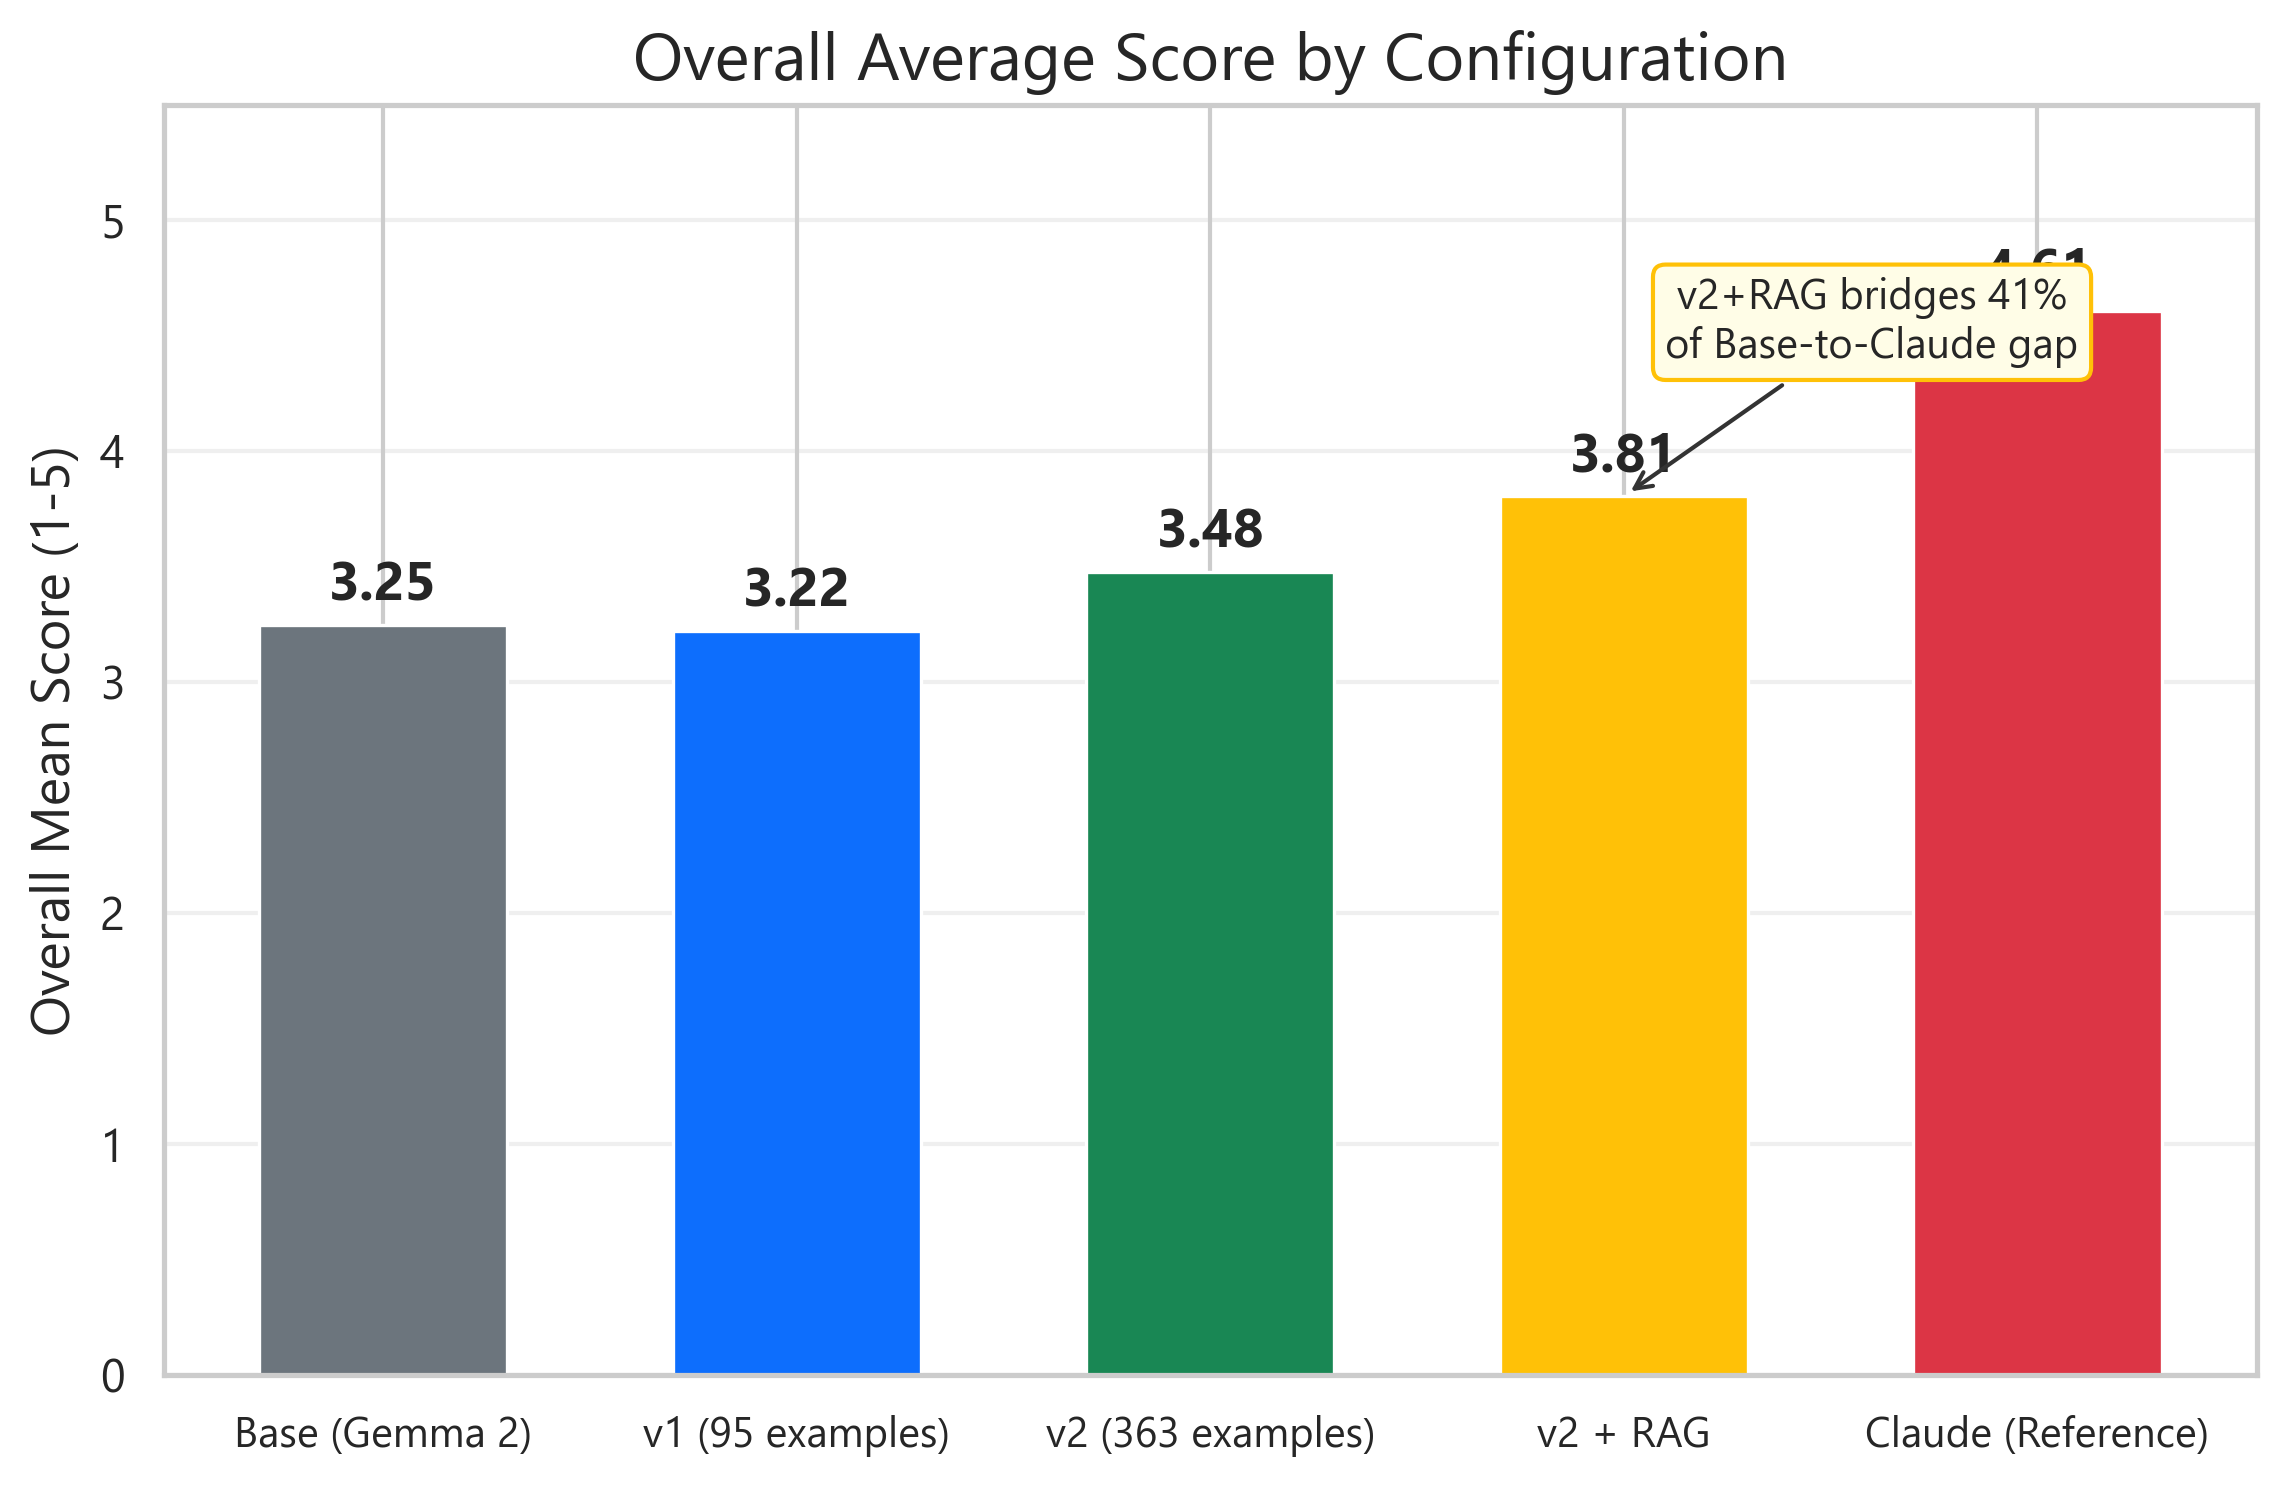
\includegraphics[width=0.78\linewidth]{05_overall_average.png}
\caption{Overall mean score (unweighted across the five MI dimensions) per
configuration. Higher is better. The fine-tuned Gemma-2-2B with RAG reaches
$3.81/5.0$, closing roughly $41\%$ of the gap between the base Gemma-2-2B
($3.25$) and Claude Haiku ($4.61$).}
\label{fig:overall}
\end{figure}

\subsection{Per-Dimension Comparison}

Aggregate numbers obscure where the gains came from. \Cref{fig:per-dim} shows
all five dimensions side by side; \Cref{fig:radar} shows the same data on a
radar chart that makes the shape of each configuration's strengths visible.

\begin{figure}[h]
\centering
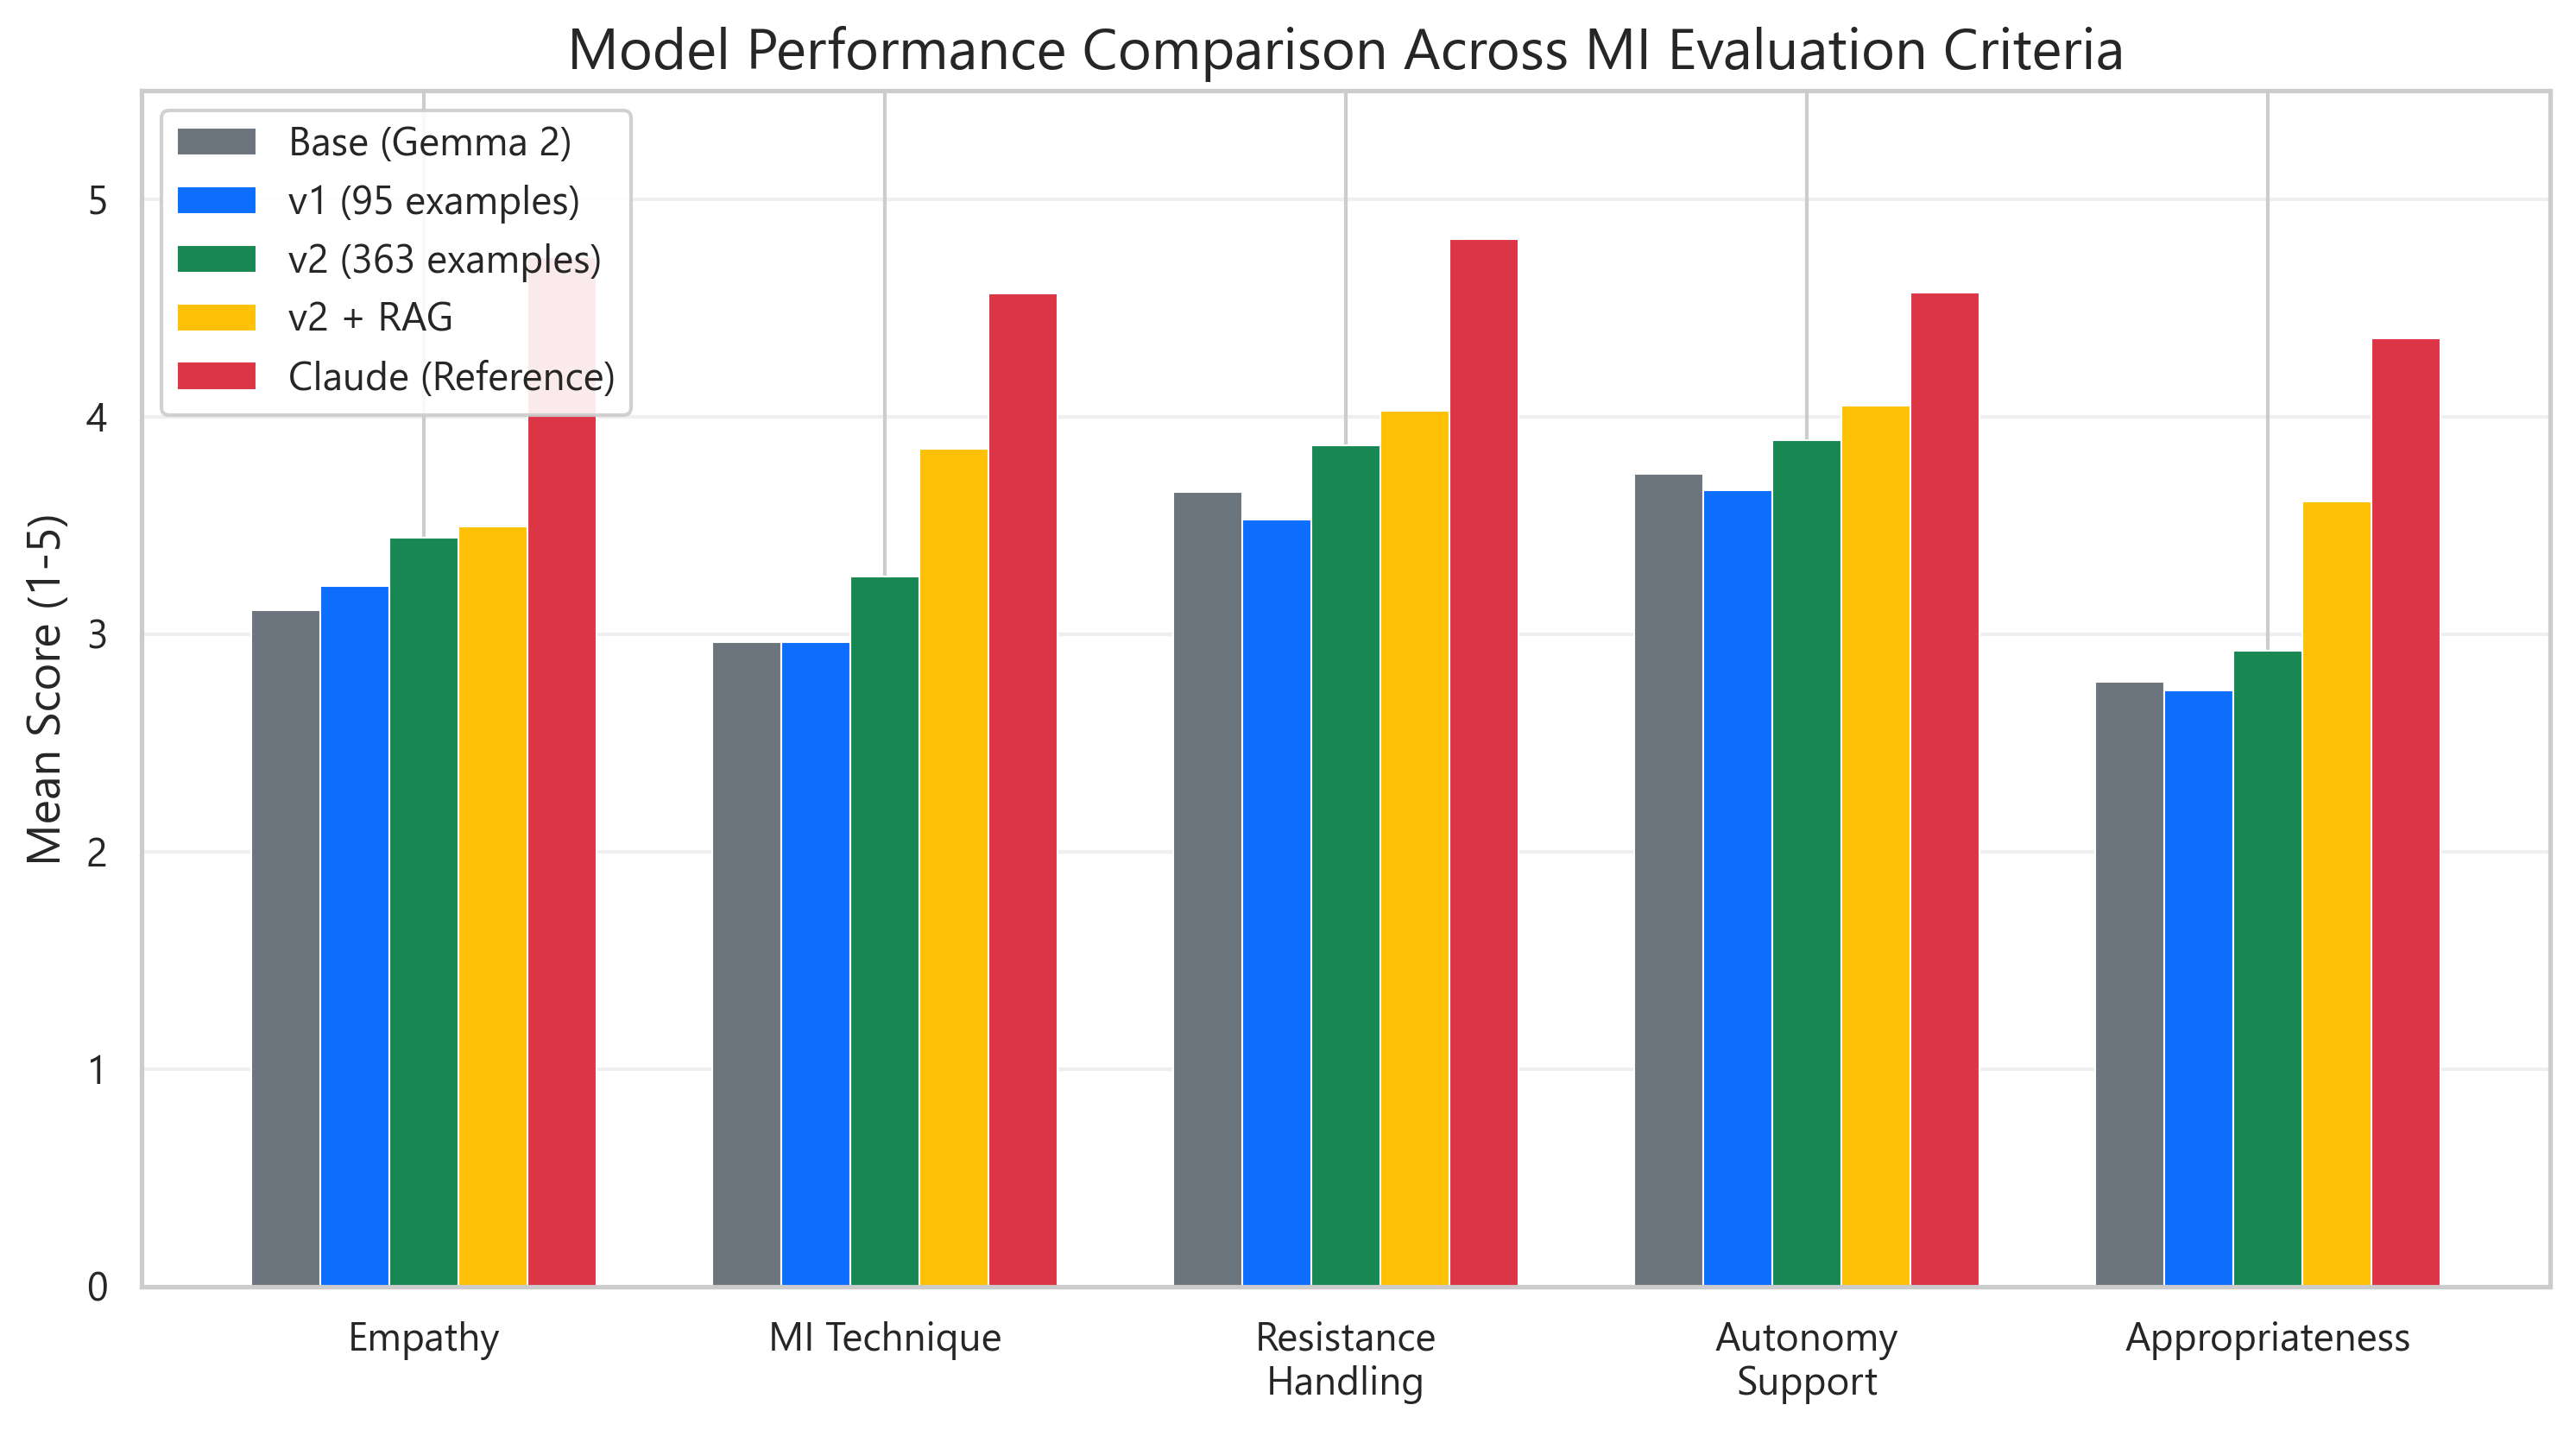
\includegraphics[width=0.92\linewidth]{01_model_comparison.png}
\caption{Per-dimension mean scores by configuration. \texttt{v2\_rag} (red)
clearly dominates the smaller-model configurations; the largest absolute gains
appear on \emph{MI technique} and \emph{appropriateness}.}
\label{fig:per-dim}
\end{figure}

\begin{figure}[h]
\centering
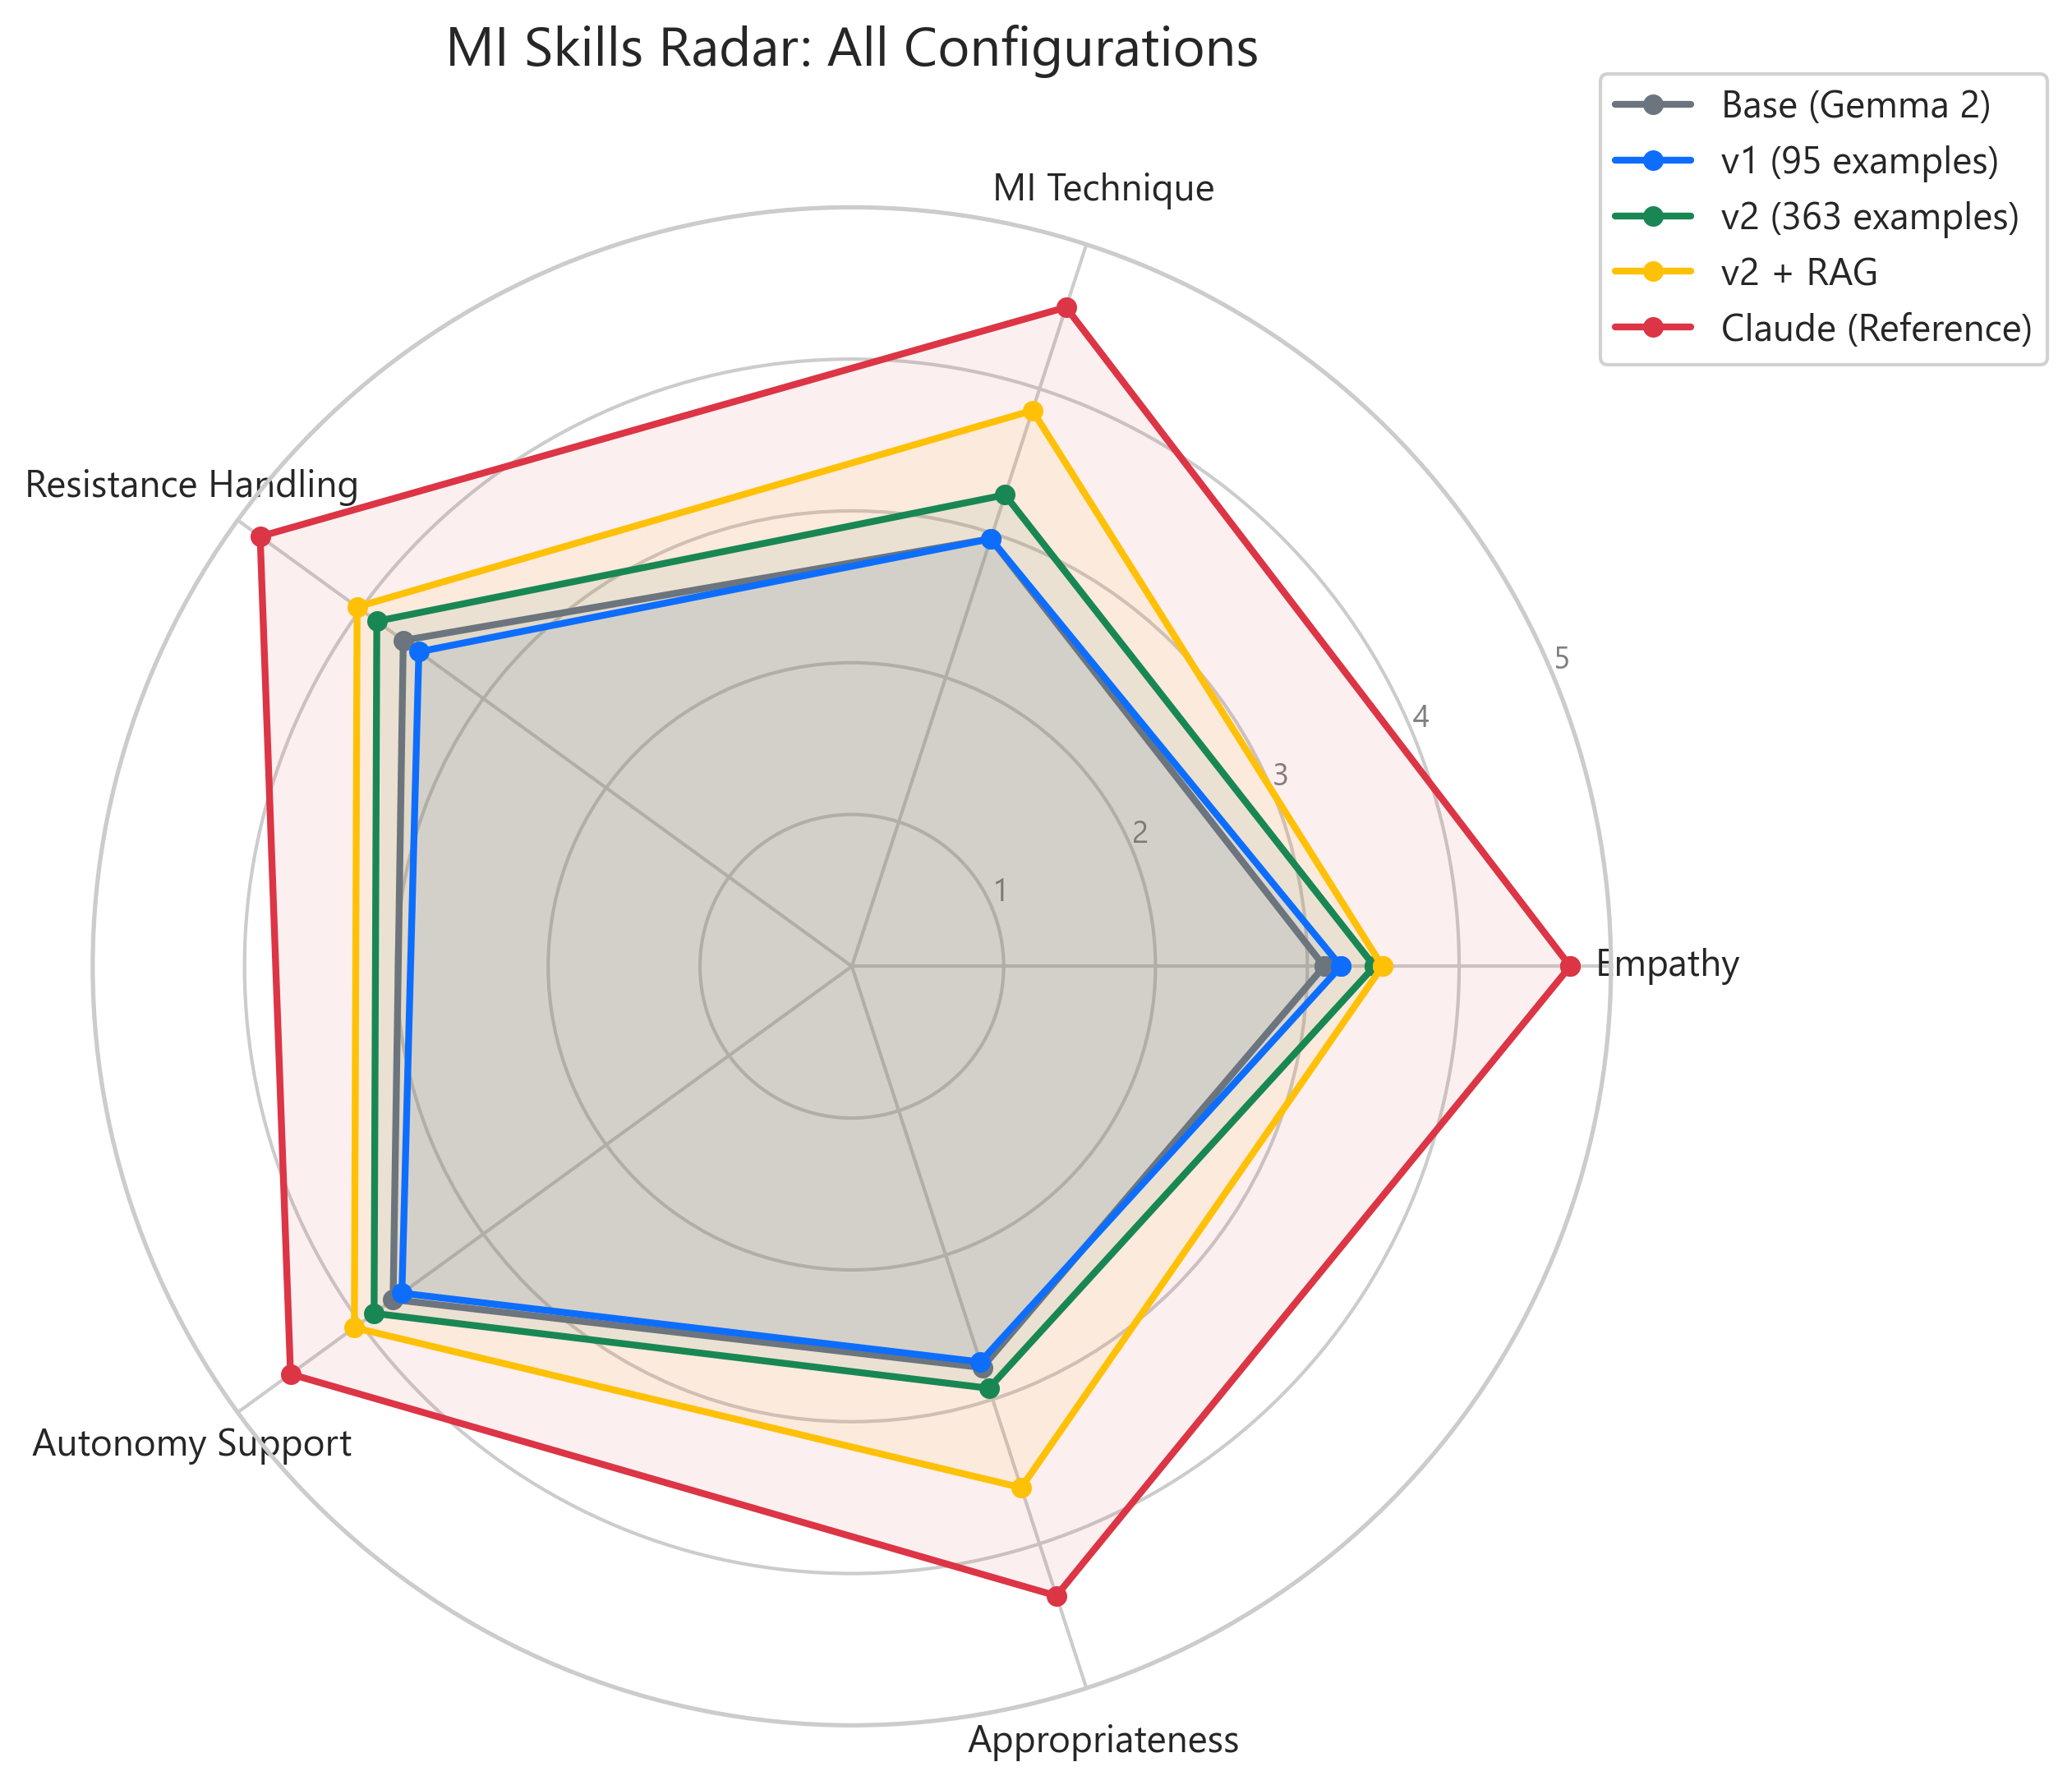
\includegraphics[width=0.62\linewidth]{02_radar_chart.png}
\caption{Radar plot of the five MI dimensions. The fine-tuned configurations
have a fundamentally different shape from \texttt{base} -- they are wider on
\emph{MI technique} and \emph{appropriateness}, the two dimensions closest to
``did the model do MI things rather than generic-assistant things''.}
\label{fig:radar}
\end{figure}

The dimension-level gains of \texttt{v2\_rag} over \texttt{base} are
summarized in \Cref{tab:per-dim-delta}.

\begin{table}[h]
\centering
\caption{Per-dimension improvement of \texttt{v2\_rag} over \texttt{base}.
The two largest gains -- MI technique ($+0.89$) and Appropriateness ($+0.83$)
-- are exactly the dimensions on which a generic instruction-tuned model is
weakest by construction.}
\label{tab:per-dim-delta}
\begin{tabular}{lccc}
\toprule
\textbf{Dimension} & \textbf{base} & \textbf{v2\_rag} & $\Delta$ \\
\midrule
Empathy             & 3.11 & 3.49 & $+0.38$ \\
MI technique        & 2.96 & 3.85 & $+0.89$ \\
Resistance handling & 3.65 & 4.03 & $+0.38$ \\
Autonomy support    & 3.73 & 4.05 & $+0.32$ \\
Appropriateness     & 2.78 & 3.61 & $+0.83$ \\
\bottomrule
\end{tabular}
\end{table}

\Cref{fig:improvement} expresses the same data as a per-dimension delta, and
\Cref{fig:heatmap} shows the full configuration $\times$ dimension matrix.

\begin{figure}[h]
\centering
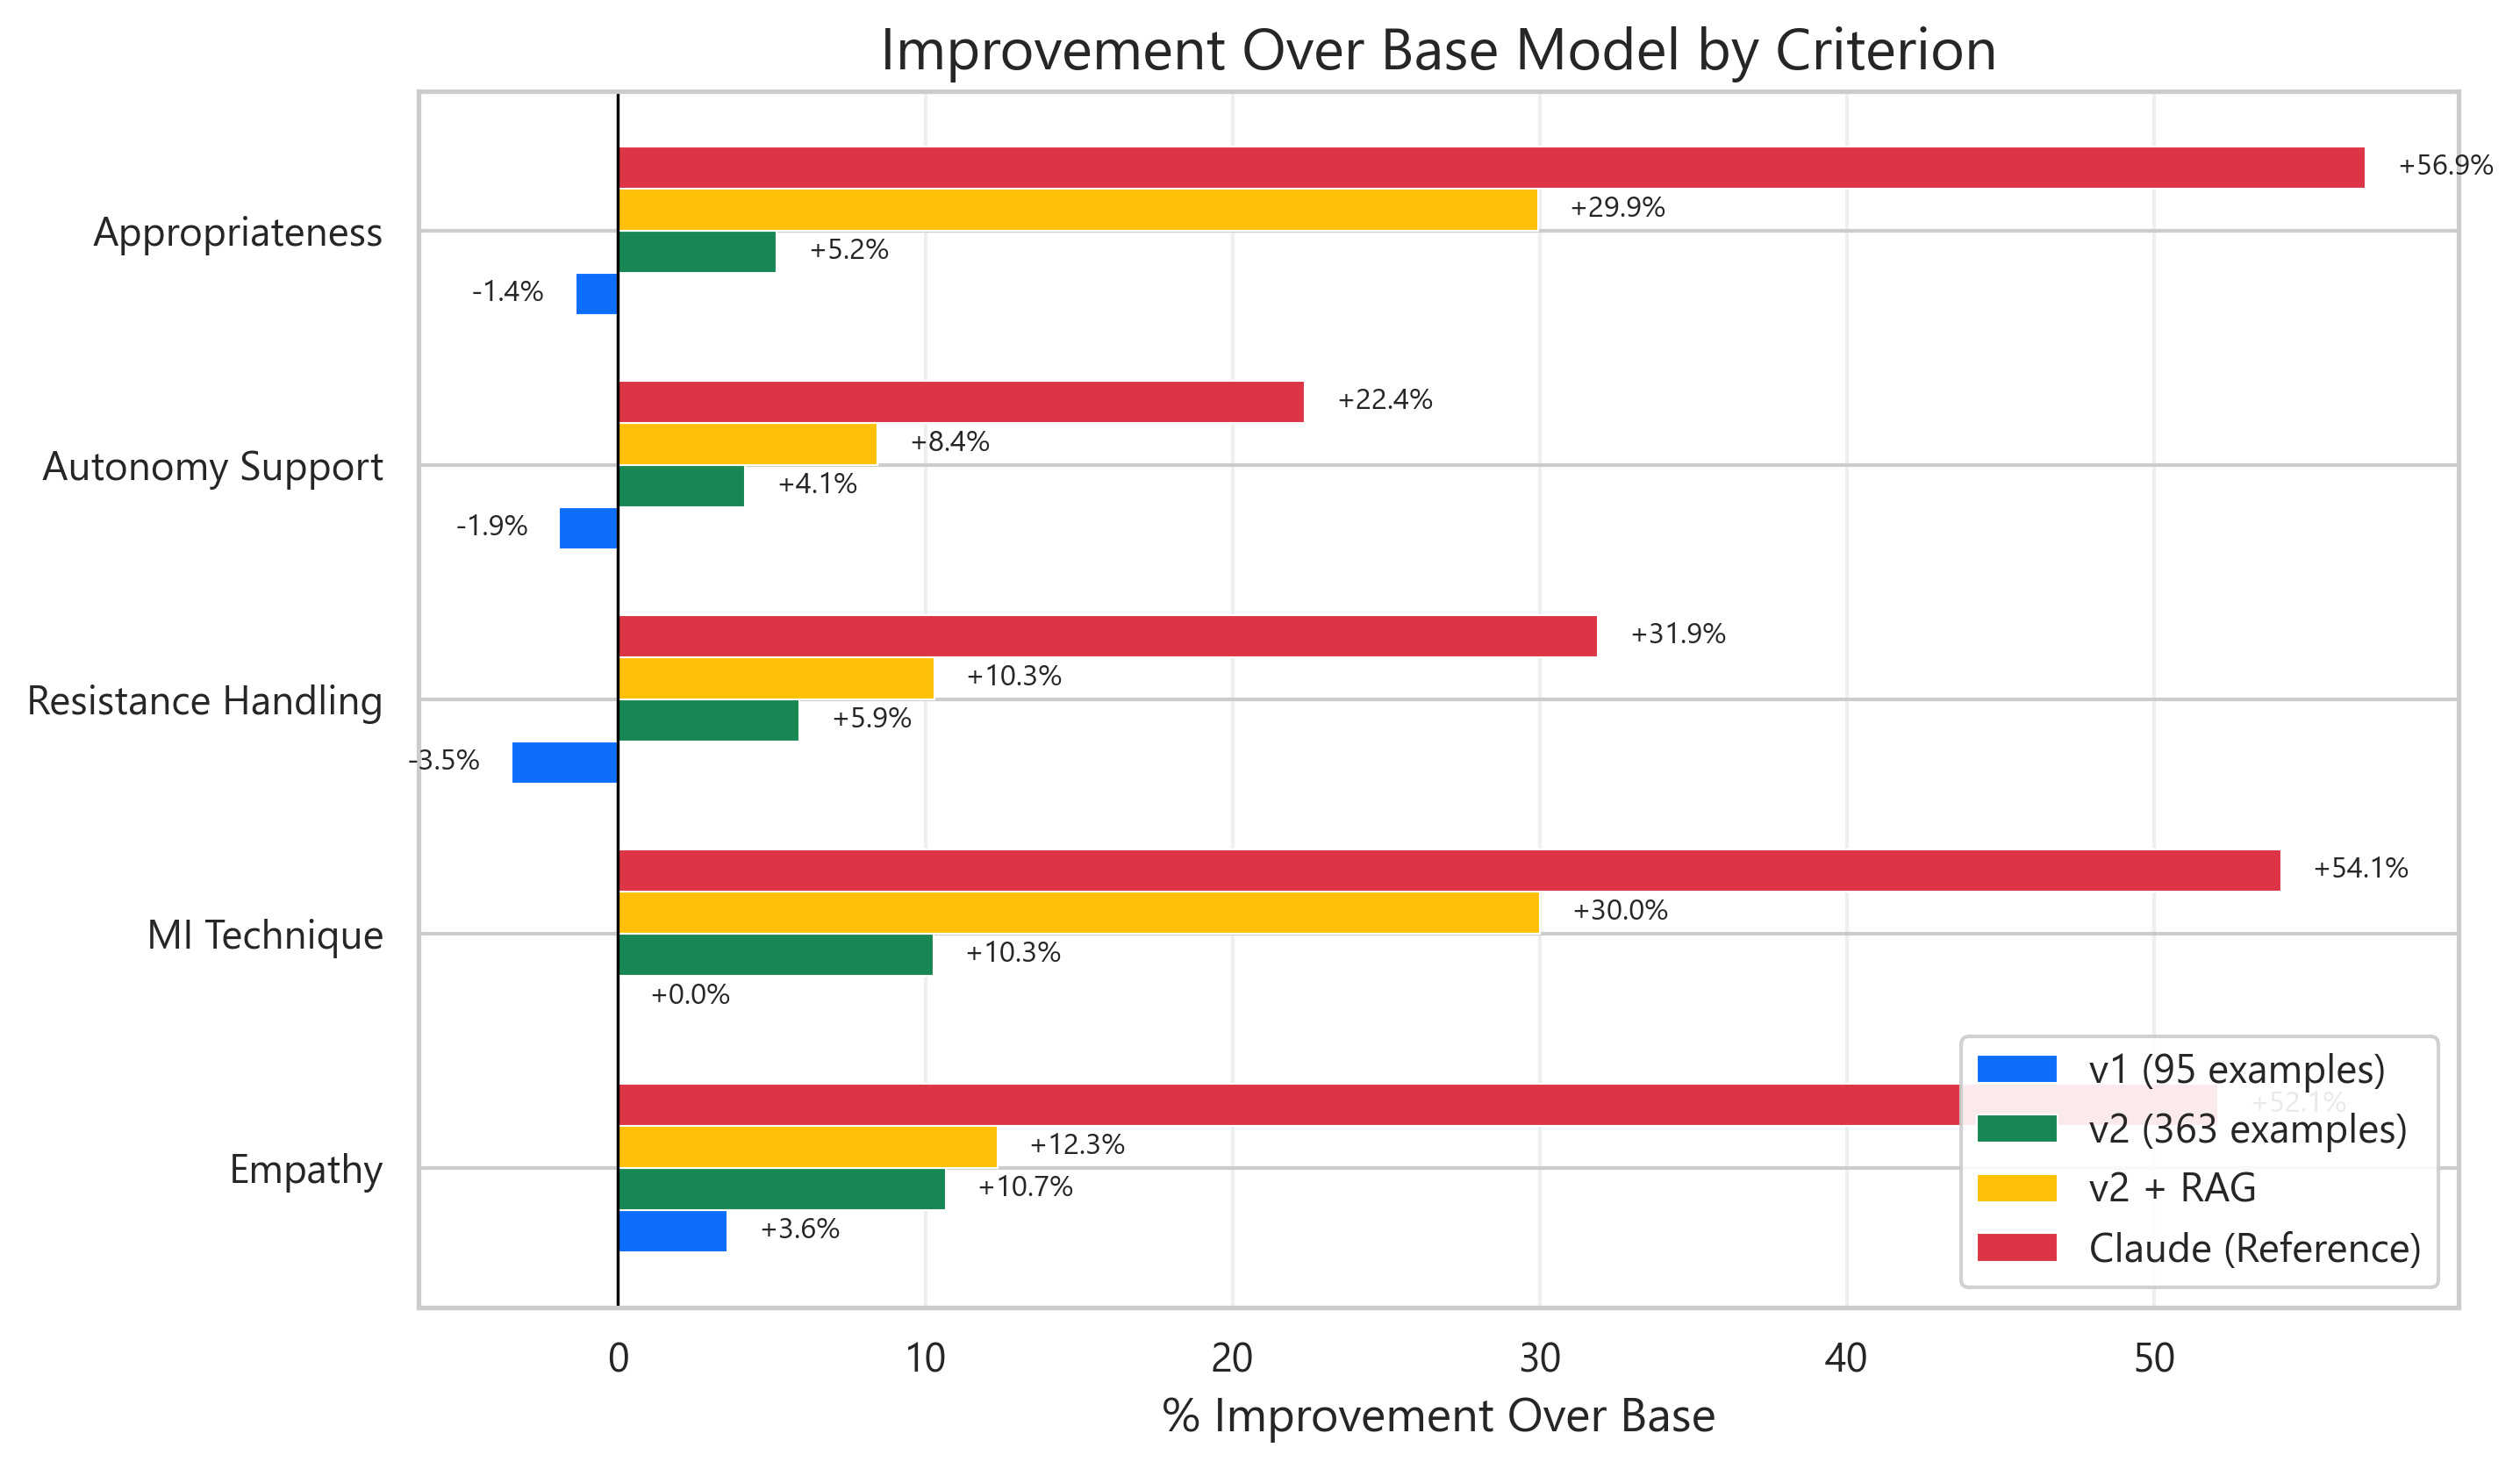
\includegraphics[width=0.78\linewidth]{03_improvement_over_base.png}
\caption{Absolute score gain of \texttt{v2\_rag} over \texttt{base}, by
dimension. The two MI-specific dimensions (technique, appropriateness) gain
nearly a full point on a 5-point scale; the more general dimensions (empathy,
resistance handling, autonomy support) gain less because the base model was
already passable on them.}
\label{fig:improvement}
\end{figure}

\begin{figure}[h]
\centering
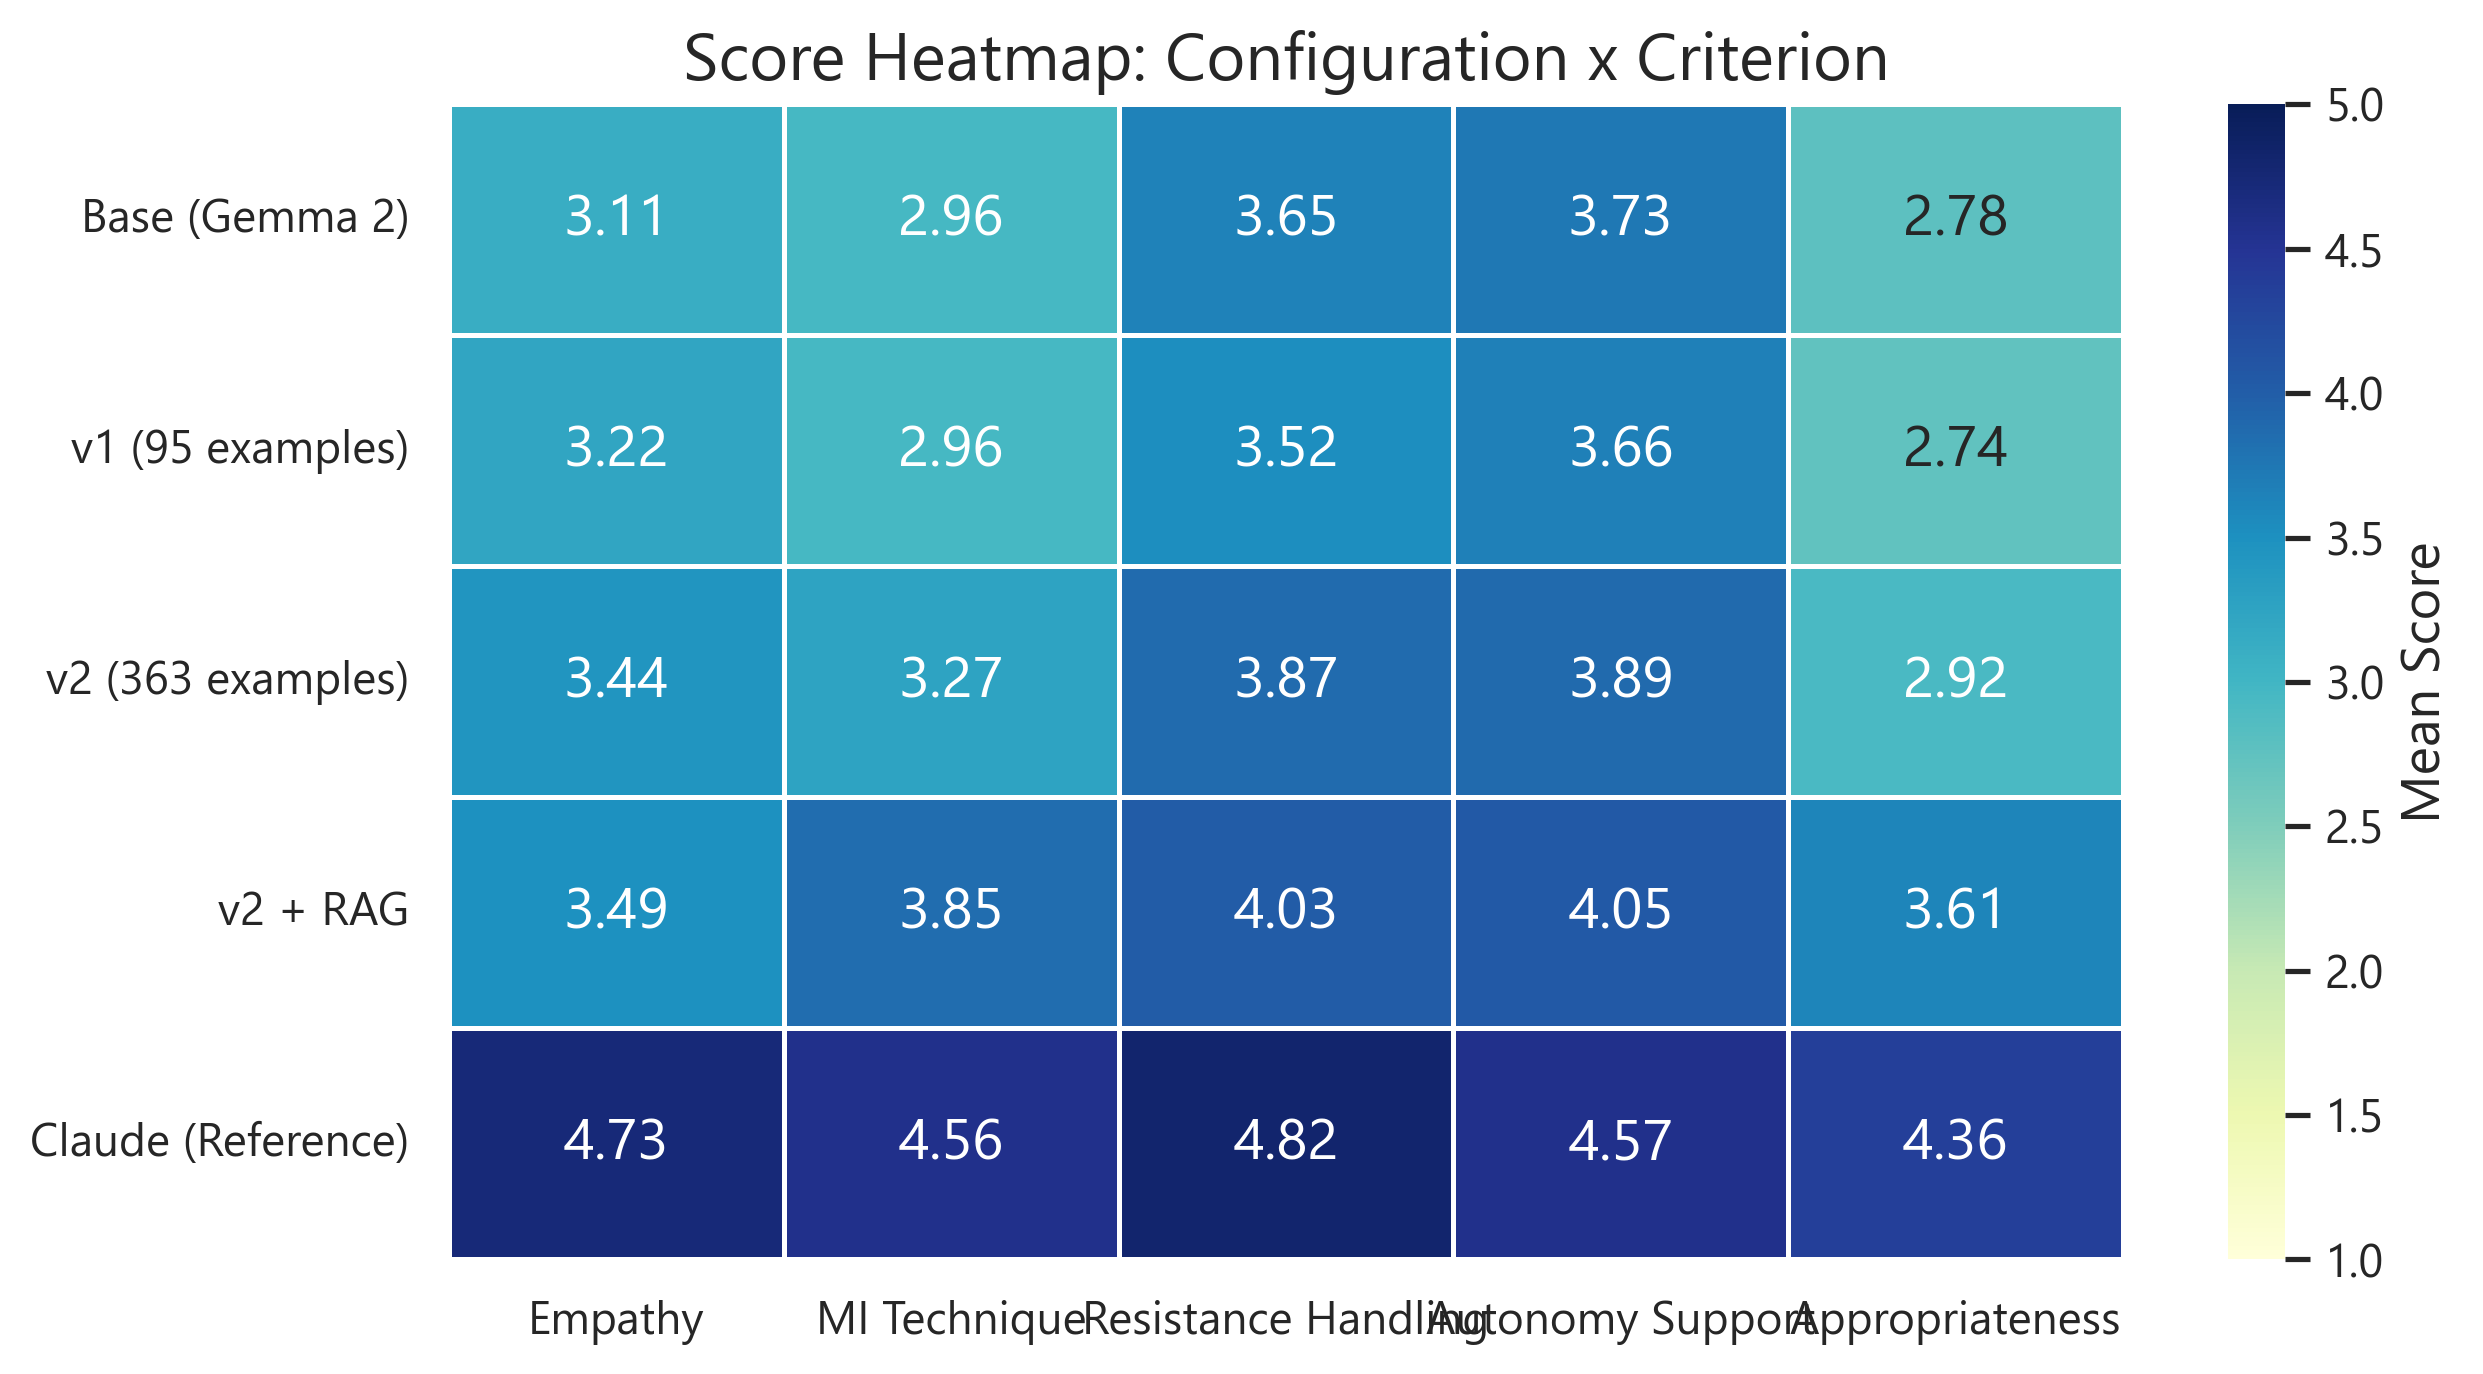
\includegraphics[width=0.85\linewidth]{06_heatmap.png}
\caption{Configuration $\times$ dimension heatmap. The visual pattern -- a
near-uniform top row for Claude, a graded gradient down the fine-tuned
configurations, and a thin top from \texttt{base} on Empathy/Resistance --
matches the per-dimension narrative.}
\label{fig:heatmap}
\end{figure}

\subsection{The v1 Result}

\Cref{tab:results-main} contains a result that deserves a sentence on its own:
\texttt{v1} (fine-tuned on real AnnoMI alcohol data \emph{only}) scores
$3.22$ overall, slightly \emph{below} \texttt{base} ($3.25$). This is a real
finding, not noise. With $\approx$363 training examples, a small instruction-tuned
model does not learn enough to compensate for the specialization cost; the
fine-tune appears to have narrowed its style without improving its MI quality.

The reason \texttt{v2} ($3.48$) clears \texttt{base} is the synthetic data:
once the training set is widened with the $\approx$1{,}000 generated
conversations covering the four scenario types, the same fine-tuning recipe
produces a meaningful gain. This is the strongest single piece of evidence
that the synthetic-data step was load-bearing rather than decorative.

\subsection{Technique Distribution}

\Cref{fig:tech} reports which MI techniques the judge actually \emph{detected}
in each configuration's responses. This is independent of score quality -- it
is a description of \emph{what} the model does, not how well.

\begin{figure}[h]
\centering
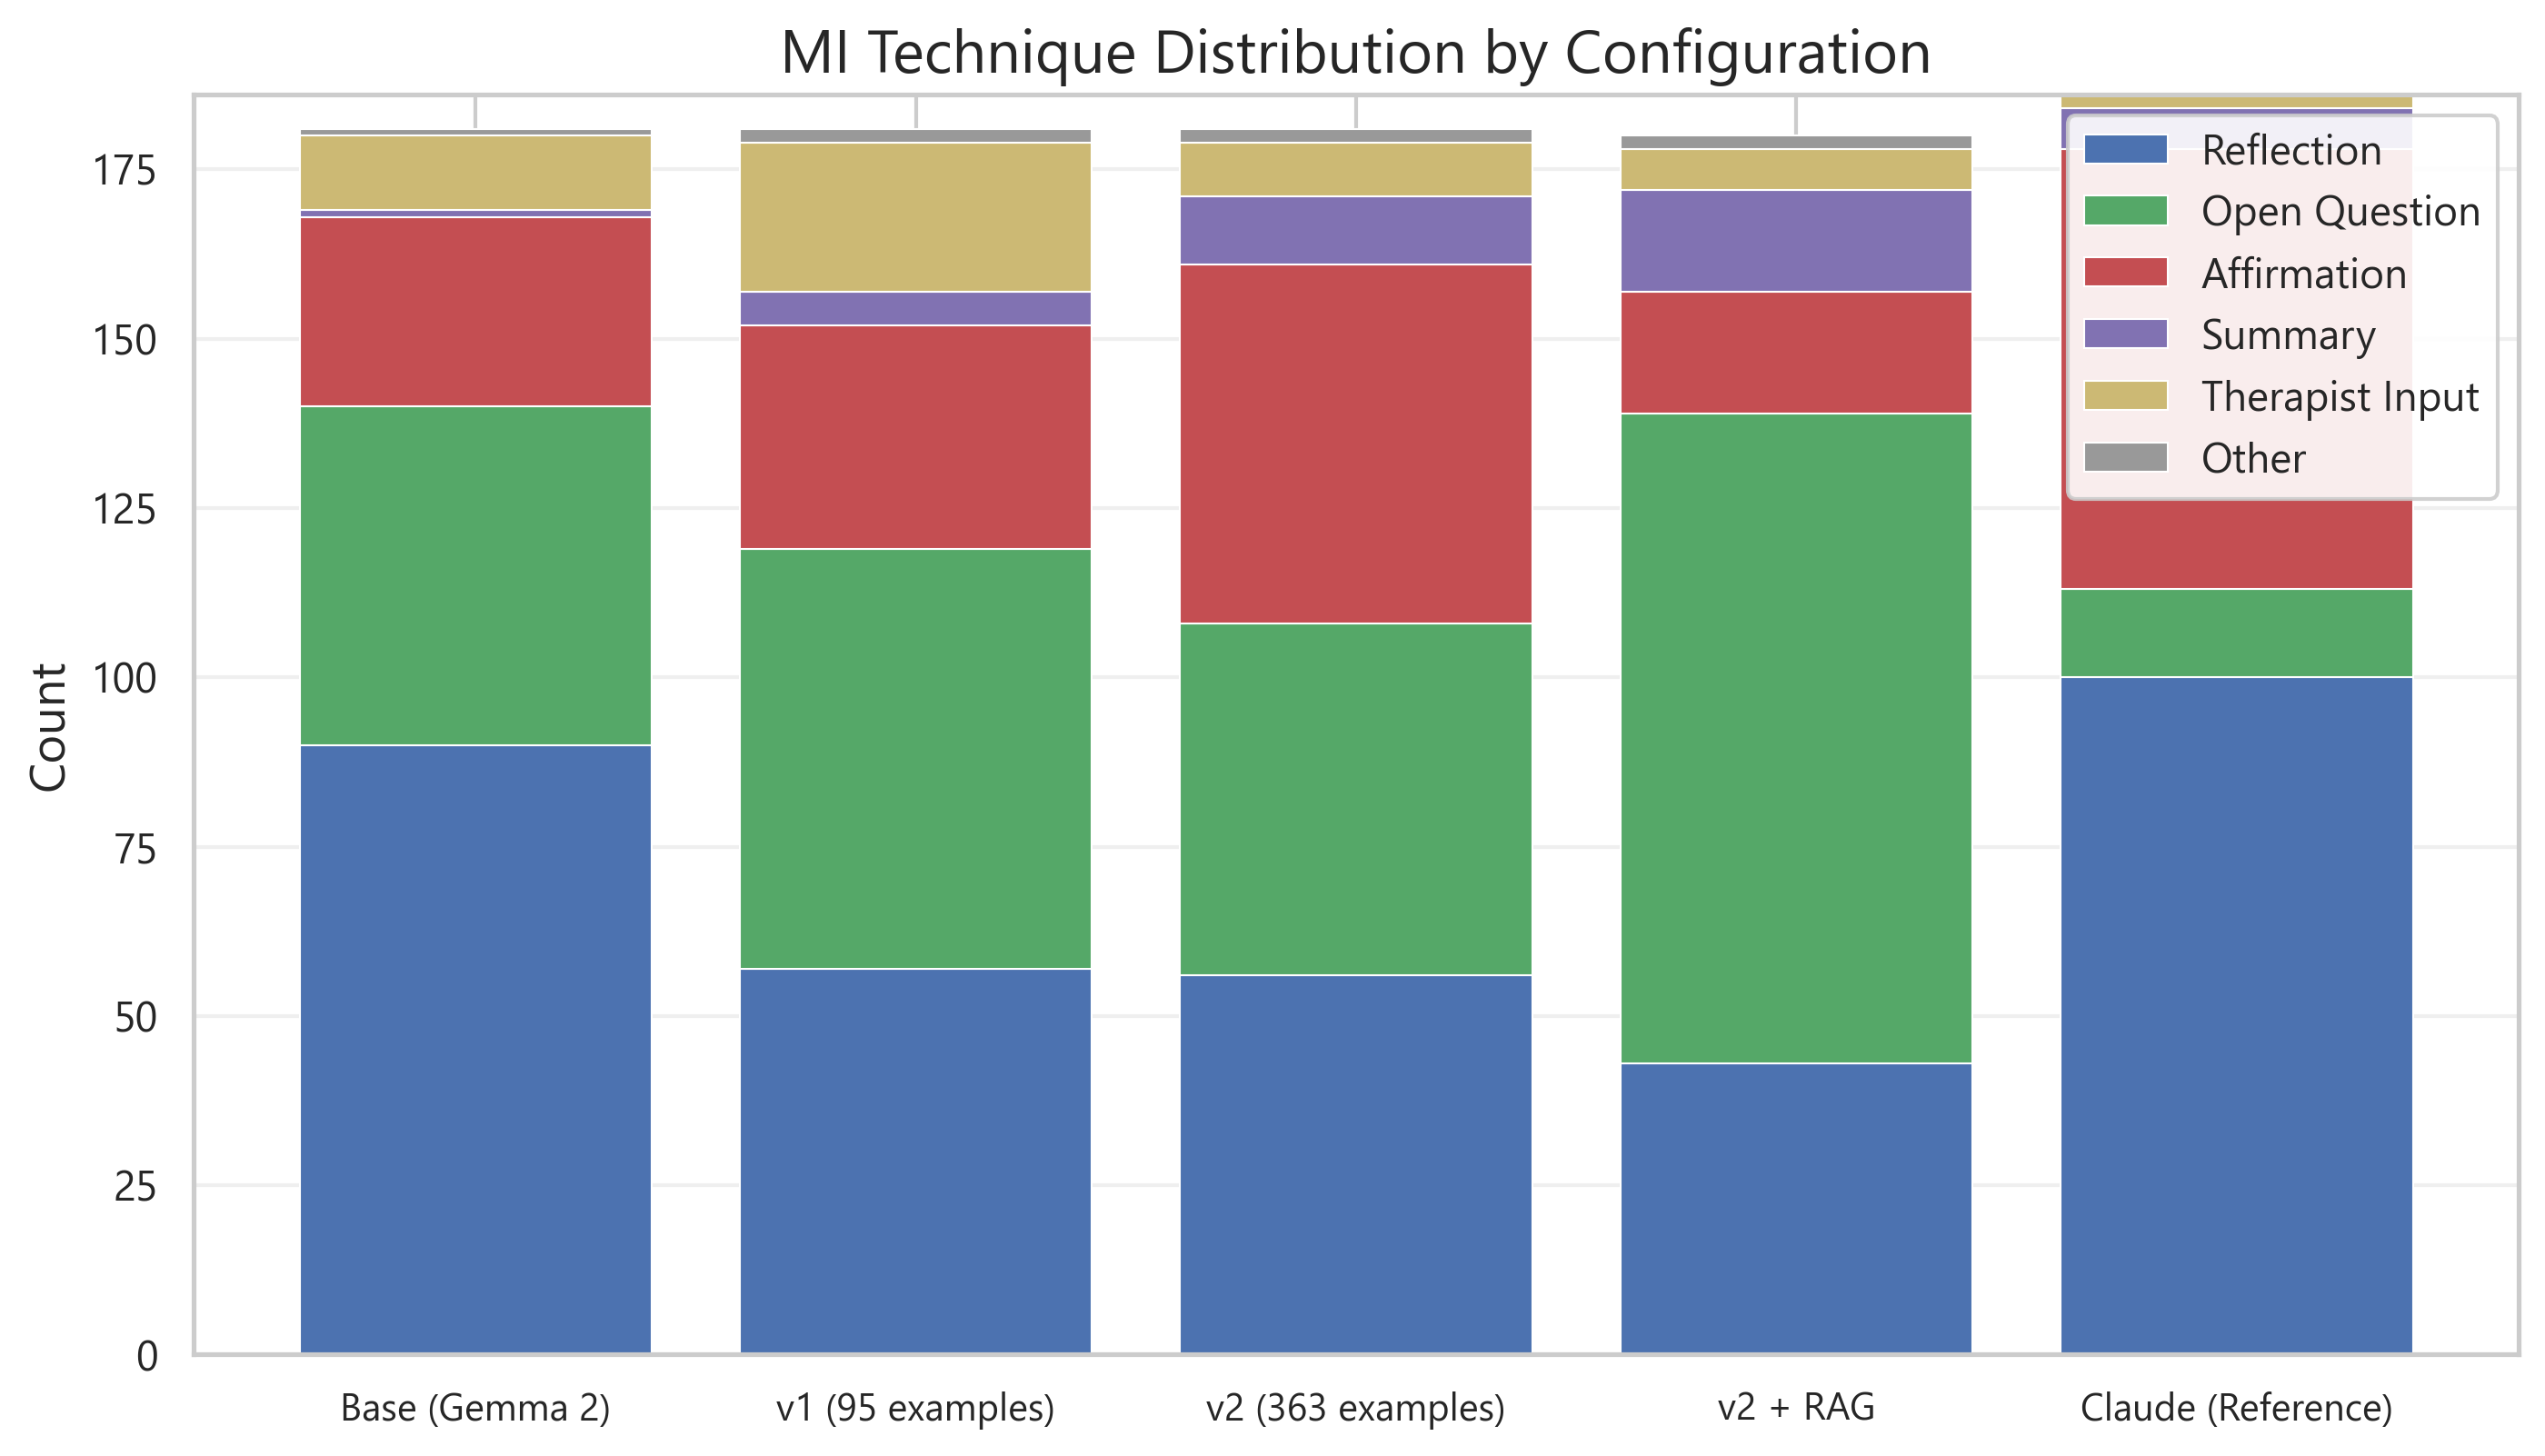
\includegraphics[width=0.92\linewidth]{04_technique_distribution.png}
\caption{Distribution of MI techniques detected by the judge per configuration.
The fine-tuned configurations shift the modal output toward
\textit{reflection}/\textit{open question} -- the canonical MI moves -- and
away from \textit{advice}/\textit{closed question}. \texttt{v2\_rag} most
closely tracks the Claude reference's distribution.}
\label{fig:tech}
\end{figure}

\subsection{Qualitative Examples}

Numbers alone do not carry the texture of what the fine-tune actually changed.
\Cref{tab:qual} shows one representative AnnoMI test turn and the response
from each configuration.

\begin{table}[h]
\centering
\caption{Representative qualitative comparison on a real AnnoMI test turn.
The user is mildly defensive; the reference response from the human counselor
uses a scaling question, a canonical MI move.}
\label{tab:qual}
\renewcommand{\arraystretch}{1.2}
\begin{tabularx}{\linewidth}{l X}
\toprule
\textbf{User turn} & \textit{``I don't really think I drink that much. My friends drink the same.''} \\
\midrule
\texttt{base}    & Highlights health risks of regular drinking and recommends tracking intake -- advice-giving, MI-inconsistent. \\
\texttt{v1}      & Asks ``how much is that, exactly?'' -- a closed quantitative question that invites further defensiveness. \\
\texttt{v2}      & Reflects: ``It sounds like comparing yourself to your friends makes it feel pretty normal.'' MI-consistent simple reflection. \\
\texttt{v2\_rag} & Reflects \emph{and} pivots to autonomy: ``It sounds normal to you, given who you're around. What would help you decide whether you wanted to think more about it -- not because anyone says so, but on your own terms?'' \\
\texttt{claude}  & A complex reflection plus a scaling question, similar in shape to the human reference. \\
\bottomrule
\end{tabularx}
\end{table}

The qualitative gradient mirrors the quantitative one: \texttt{base} gives
advice, \texttt{v1} reverts to closed questioning, \texttt{v2} reaches a
correct simple reflection, and \texttt{v2\_rag} layers a reflection with an
autonomy-supporting follow-up that reads as deliberate MI rather than
templated.

\subsection{Latency and Footprint}

\Cref{tab:latency} reports inference characteristics on the deployment target.
Latency was measured end-to-end (full pipeline including state inference and
RAG retrieval) on a CPU-only laptop, averaged over 50 turns of the eval set.

\begin{table}[h]
\centering
\caption{Inference characteristics of the deployed configurations.
Footprint is the on-disk model artifact; latency is full end-to-end per turn
on CPU including pipeline overhead.}
\label{tab:latency}
\begin{tabular}{lcc}
\toprule
\textbf{Configuration} & \textbf{Footprint} & \textbf{Latency (CPU)} \\
\midrule
\texttt{base / v1 / v2 / v2\_rag} (Gemma-2-2B Q4\_K\_M GGUF) & $\sim$1.6 GB & $\sim$2--4 s \\
\texttt{claude} (Haiku via API)                              & N/A (hosted) & $\sim$1--2 s \\
\bottomrule
\end{tabular}
\end{table}

The 2--4 s latency is acceptable for a demo and fine for the evaluation loop
but is too slow for a fluent real-time conversation -- a limitation discussed
further in \Cref{sec:future_work}.

\subsection{Summary}

The headline findings are:
\begin{enumerate}
    \item Fine-tuning a 2B-parameter open-weights model with LoRA on a mixed
    real + synthetic MI corpus and adding RAG over a curated MI knowledge base
    closes $\approx$41\% of the gap to a much larger Claude Haiku reference,
    with an absolute gain of $+0.56$ ($+17.2\%$ relative) over the
    no-fine-tune baseline.
    \item The largest gains are on \emph{MI technique} ($+0.89$) and
    \emph{appropriateness} ($+0.83$) -- precisely the dimensions on which a
    generic instruction-tuned model is weakest.
    \item Fine-tuning on real AnnoMI \emph{alone} ($\sim$363 examples) is
    not enough; the synthetic-data augmentation step is load-bearing.
    \item Adding RAG to the v2 fine-tune yields a further $+0.33$ overall,
    confirming that knowledge retrieval is complementary to fine-tuning rather
    than redundant with it.
    \item The headline gap to a much larger model remains substantial
    ($-0.80$ overall on a 5-point scale), as expected; the project's claim is
    not parity but rather that a small, locally-deployable model can be moved
    into a usable MI-consistent regime.
\end{enumerate}

\section{Conclusions}
\label{sec:conclusions}

This capstone designed, implemented, and evaluated a six-stage pipeline for an
MI-aligned chatbot for alcohol-related dialogues. The headline result is that
a parameter-efficient fine-tune of \texttt{gemma-2-2b-it}, trained on the
AnnoMI alcohol-only subset augmented with $\approx$1{,}000 synthetic MI
conversations and supplemented at inference time by retrieval over a curated
MI knowledge base, reaches an LLM-as-judge score of $3.81/5.0$ on a
181-item evaluation set spanning real, synthetic, and edge-case turns. That
is a $+17.2\%$ relative improvement over the base model and closes $41\%$
of the absolute gap to a much larger Claude Haiku reference.

Beyond the headline number, four conclusions are worth stating explicitly.

\subsubsection*{1. Synthetic data was load-bearing, not decoration.}
Fine-tuning on AnnoMI alone (\texttt{v1}) did not improve over the base model;
in fact it nudged the overall score slightly down. Only after the training set
was widened with synthetic dialogue covering scenario shapes the real data
under-covers (long sessions, mixed defensiveness within a session) did the
fine-tune produce a meaningful gain (\texttt{v2}). The lesson is that for
small specialized corpora, ``just train on the real data'' is not enough --
the model needs enough \emph{shape} variety to learn a stylistic identity, and
synthetic generation is one practical way to provide it.

\subsubsection*{2. Retrieval is complementary to fine-tuning, not redundant.}
\texttt{v2\_rag} adds $+0.33$ on top of \texttt{v2}, which is more than the
fine-tune itself contributed over the base. This says that the model and the
knowledge base were doing genuinely different work: fine-tuning shaped
\emph{how} the model talks; retrieval gave it the right \emph{what} to say in
a given turn. Treating them as substitutes -- a common temptation when
budgets are tight -- would have left meaningful quality on the table.

\subsubsection*{3. Auditability needs to be a first-class design choice.}
The decision to make safety a regex screen plus per-turn JSONL audit logging
-- rather than an embedding-based classifier and an ephemeral runtime --
paid off twice in the project: once when the original strict-adjacency
crisis patterns were found to miss natural phrasings, and once when the
debugging affordance of the per-turn log made it possible to reconstruct
exactly which retrieved chunks the model was conditioned on for any given
output. Both fixes were one-commit changes against an inspectable surface;
neither would have been against an opaque classifier or an unlogged runtime.

\subsubsection*{4. LLM-as-judge is fine for iteration, not for adjudication.}
The five-dimension rubric and the $\approx$181-item evaluation set produced a
signal stable enough to drive iteration -- the consistent ordering of
\texttt{base $<$ v2 $<$ v2\_rag $<$ claude} across configurations, runs, and
dimensions is itself evidence of internal consistency. But this is not a
clinical adjudication. The scores correlate with human MI ratings only in the
coarse sense documented by \cite{zheng2023judging,chiang2023closer}, and the
project treats them as that: a coarse iteration signal.

\subsection*{What This Project Demonstrates}

The combined system demonstrates that a small, locally-deployable language
model can be moved from ``general-purpose assistant that defaults to
advice-giving'' into ``MI-consistent reflective interlocutor'' through a
specific stack of design choices: parameter-efficient fine-tuning on real +
synthetic data, retrieval over a curated knowledge base, two-stage regex
safety, per-turn audit logging, and a single shared pipeline behind two
purpose-fit front ends. None of those moves are individually novel; the
contribution is the integration and the honest evaluation.

\subsection*{What This Project Is Not}

It is not a clinical product. It is not validated under an institutional
review board. It is not appropriate for unsupervised deployment to people in
acute distress. The system was designed and evaluated as a research artifact
for a capstone course; the limitations and the work required to take it
further are spelled out in \Cref{sec:future_work}.

\section{Recommended Future Work}
\label{sec:future_work}

The system is functional and the headline numbers are consistent, but there
are seven directions in which the work would extend naturally. They are
ordered roughly by ratio of expected impact to effort.

\subsection{Human Evaluation}
The strongest single follow-up is a small-N human evaluation by trained MI
clinicians, even on the order of 20--30 dialogues, to calibrate the
LLM-as-judge scores to clinician judgement. The current evaluation is a
proxy; the next claim worth making about this system is one that survives
contact with a human rater.

\subsection{Larger Base Model}
The Gemma-2-2B base was chosen for local CPU deployability, and the
evaluation shows a substantial residual gap to the Claude Haiku reference.
A direct experiment is to fine-tune Gemma-2-9B (or a similarly sized
\texttt{Llama-3.1-8B-Instruct}) with the same LoRA recipe on the same data
and measure how much of the remaining gap closes. The trade-off is latency:
9B-class models are GPU-required for interactive use, so this becomes a
hosted-inference deployment rather than a local-CPU one.

\subsection{Embedding-Based Safety Classifier (as a Layer, not a Replacement)}
The current safety screen is regex-based by deliberate choice for
auditability. But regex coverage is enumerative -- semantically equivalent
phrasings can slip through. A reasonable architecture is to add an
embedding-based classifier as a \emph{second} safety layer, run only when
the regex screen passes; if the classifier flags the turn at high confidence,
the system would conservatively short-circuit to the crisis response. This
preserves regex auditability for the explicitly-listed cases while widening
coverage for paraphrases. Training data is the bottleneck: a labeled crisis
corpus would be needed and is not freely available.

\subsection{Multi-Turn Coherence}
The current evaluation scores responses turn-by-turn against per-turn
references. MI is a multi-turn process -- summaries, change-talk
elicitation, and stage-of-change progression all unfold across many turns.
A natural extension is to evaluate at the conversation level: does the
system summarize at the right moments, does it elicit and then reflect change
talk, does it avoid bringing up barriers prematurely? This requires a
conversation-level rubric and a different judge prompt structure.

\subsection{Cross-Session Memory}
The system is currently stateless across sessions -- each conversation starts
fresh. For real use this is a meaningful gap, since MI is most effective
across multiple sessions where the counselor remembers prior commitments and
prior reasons-for-change. A practical next step is per-user persistent memory
of (a) explicitly stated reasons-for-change and (b) self-reported milestones,
gated by user consent and excluded from the model's general context window
to avoid prompt bloat.

\subsection{Latency}
The 2--4~s per-turn latency on CPU is workable for demos but breaks the
conversational flow of MI in real-time use. Three independent tactics would
reduce this: (a) further quantization (Q4\_0 or Q3\_K\_S) at a small quality
cost, (b) speculative decoding via a smaller draft model, and (c) GPU
deployment with continuous batching. (a) is the cheapest experiment.

\subsection{Broader Domain Coverage}
The project is scoped to alcohol use specifically. The same pipeline -- swap
the knowledge base, refit the synthetic generator's scenario types, and
re-fine-tune -- should generalize to other behavioral-health domains for
which MI is appropriate (smoking cessation, gambling, dietary change). This
is mostly an integration question rather than a research one. The interesting
research question alongside it is how much of the alcohol-trained model's
behavior transfers across domains zero-shot, and whether a single
multi-domain fine-tune outperforms domain-specific ones at the size budget
considered here.


% =====================================================================
%  REFERENCES
% =====================================================================
\bibliographystyle{IEEEtran}
\bibliography{references}

\end{document}
